\documentclass[a4paper,14pt,oneside,final]{report}

\usepackage[utf8]{inputenc}
\usepackage[english,main=russian]{babel}
\usepackage[T1,T2A]{fontenc}
%\usepackage{pscyr}
%\renewcommand{\rmdefault}{cmr}
\usepackage[final,hidelinks]{hyperref}
\usepackage[square,numbers,sort&compress]{natbib}
%\usepackage{times}
\usefont{T2A}{ftm}{m}{sl}
\setlength{\bibsep}{0em}
\PassOptionsToPackage{hyphens}{url}

\usepackage{hyphenat}

% Курсив и жирность для кириллицы
\usepackage{substitutefont}

\substitutefont{T2A}{\familydefault}{Tempora-TLF}
\makeatletter
\input{t2atempora-tlf.fd}
\DeclareFontShape{T2A}{Tempora-TLF}{m}{sc}{
         <-> ssub * Tempora-TLF/m/n
}{}

\addto\extrasrussian{%
  \def\equationautorefname{формула}%
  \def\figureautorefname{рисунок}%
  \def\listingautorefname{листинг}%
  \def\tableautorefname{таблица}%
}

\addto\captionsrussian{
  \renewcommand\contentsname{\centerline{\bfseries\large{\MakeUppercase{Содержание}}}}
  \renewcommand{\bibsection}{\sectioncentered*{Cписок использованных источников}}
  \renewcommand{\listingscaption}{Листинг}
}

\AtEndDocument{

  \addcontentsline{toc}{section}{Cписок использованных источников}%
}
\usepackage{extsizes}


\sloppy

\usepackage{microtype}
\newlength{\fivecharsapprox}
\setlength{\fivecharsapprox}{6ex}


\usepackage{indentfirst}
\setlength{\parindent}{\fivecharsapprox} 

\usepackage[left=3cm,top=2.0cm,right=1.5cm,bottom=2.7cm]{geometry}

\frenchspacing

\usepackage{perpage}
\MakePerPage{footnote}

\makeatletter 
\def\@makefnmark{\hbox{\@textsuperscript{\normalfont\@thefnmark)}}}
\makeatother

\usepackage[bottom]{footmisc}

\makeatletter
\renewcommand{\thesection}{\arabic{section}}
\makeatother

\setcounter{secnumdepth}{3}


% Зачем: Настраивает отступ между таблицей с содержанимем и словом СОДЕРЖАНИЕ
\usepackage{tocloft}
\setlength{\cftbeforetoctitleskip}{-1em}
\setlength{\cftaftertoctitleskip}{1em}


% Зачем: Определяет отступы слева для записей в таблице содержания.
\makeatletter
\renewcommand{\l@section}{\@dottedtocline{1}{0.5em}{1.2em}}
\renewcommand{\l@subsection}{\@dottedtocline{2}{1.7em}{2.0em}}
\makeatother


% Зачем: Работа с колонтитулами
\usepackage{fancyhdr} 
\pagestyle{fancy}


\fancyhf{} 
\fancyfoot[R]{\thepage}
\renewcommand{\footrulewidth}{0pt} 
\renewcommand{\headrulewidth}{0pt}
\fancypagestyle{plain}{ 
    \fancyhf{}
    \rfoot{\thepage}}


% Зачем: Задает стиль заголовков раздела жирным шрифтом, прописными буквами, без точки в конце
\makeatletter
\renewcommand\section{%
  \@startsection {section}{1}%
    {\fivecharsapprox}%
    {-1em \@plus -1ex \@minus -.2ex}%
    {1em \@plus .2ex}%
    {\raggedright\hyphenpenalty=10000\normalfont\bfseries\MakeUppercase}}
\makeatother


% Зачем: Задает стиль заголовков подразделов

\makeatletter
\renewcommand\subsection{
  \@startsection{subsection}{2}
    {\fivecharsapprox}
    {-1em \@plus -1ex \@minus -.2ex}
    {1em \@plus .2ex}
    {\raggedright\hyphenpenalty=10000\normalfont\normalsize\bfseries}}
\makeatother


% Зачем: Задает стиль заголовков пунктов
\makeatletter
\renewcommand\subsubsection{
  \@startsection{subsubsection}{3}%
    {\fivecharsapprox}%
    {-1em \@plus -1ex \@minus -.2ex}%
    {\z@}%
    {\raggedright\hyphenpenalty=10000\normalfont\normalsize\bfseries}}
\makeatother

% Зачем: для оформления введения и заключения, они должны быть выровнены по центру.
\makeatletter
\newcommand\sectioncentered{%
  \clearpage\@startsection {section}{1}%
    {\z@}%
    {-1em \@plus -1ex \@minus -.2ex}%
    {1em \@plus .2ex}%
    {\centering\hyphenpenalty=10000\normalfont\large\bfseries\MakeUppercase}%
    }
\makeatother



% Зачем: Задает стиль библиографии
\bibliographystyle{gost71s2003}

\usepackage[final]{graphicx}
\DeclareGraphicsExtensions{.png,.jpg}

% Зачем: Добавление подписей к рисункам
\usepackage{caption}
\usepackage{subcaption}

% Зачем: поворот ячеек таблиц на 90 градусов
\usepackage{rotating}
\DeclareRobustCommand{\povernut}[1]{\begin{sideways}{#1}\end{sideways}}

\DeclareRobustCommand{\x}[1]{\text{#1}}

% Зачем: Задание подписей, разделителя и нумерации частей рисунков
\DeclareCaptionLabelFormat{stbfigure}{Рисунок \emph{#2}}
\DeclareCaptionLabelFormat{stbtable}{Таблица \emph{#2}}
\DeclareCaptionLabelFormat{stblisting}{Листинг \emph{#2}}
\DeclareCaptionLabelSeparator{stb}{~--~}
\captionsetup{labelsep=stb}
\captionsetup[figure]{labelformat=stbfigure, justification=centering, font={small}}
\captionsetup[listing]{labelformat=stblisting,justification=centering, font={small}}
\captionsetup[table]{labelformat=stbtable,justification=raggedright,  font={small}}
\renewcommand{\thesubfigure}{\asbuk{subfigure}}
% Зачем: Окружения для оформлени<я формул
\usepackage{calc}
\newlength{\lengthWordWhere}
\settowidth{\lengthWordWhere}{где}
%\newenvironment{explanation}
 %   {
 %   \begin{itemize}[leftmargin=0cm, itemindent=\lengthWordWhere + \labelsep , labelsep=\labelsep]

 %   \renewcommand\labelitemi{}
    %}
    %{
    %\\[\parsep]
    %\end{itemize}
    %}


\usepackage{tabularx}

\newenvironment{explanationx}
    {
    \noindent 
    \tabularx{\textwidth}{@{}ll@{ --- } X }
    }
    { 
    \\[\parsep]
    \endtabularx
    }

\usepackage{amsmath}

\usepackage{amsfonts}
\usepackage{amssymb}
\usepackage{amsthm}
\usepackage{calc}
\usepackage{fp}
\usepackage{enumitem}

\makeatletter
 \AddEnumerateCounter{\asbuk}{\@asbuk}{щ)}
\makeatother


\setlist{nolistsep}
\renewcommand{\labelenumi}{\arabic{enumi}.}
\renewcommand{\labelenumii}{\alph{enumii}.}

%\setlist[itemize,0]{itemindent=\parindent + 2.2ex,leftmargin=0ex,label=--}
%\setlist[enumerate,1]{leftmargin=4em}
%\setlist[enumerate,2]{leftmargin=0em}


% Зачем: Включение номера раздела в номер формулы. Нумерация формул внутри раздела.
\AtBeginDocument{\numberwithin{equation}{section}}

% Зачем: Включение номера раздела в номер таблицы. Нумерация таблиц внутри раздела.
\AtBeginDocument{\numberwithin{table}{section}}

% Зачем: Включение номера раздела в номер рисунка. Нумерация рисунков внутри раздела.
\AtBeginDocument{\numberwithin{figure}{section}}

% Зачем: Включение номера раздела в номер листинга. Нумерация листингов внутри раздела.
\AtBeginDocument{\numberwithin{listing}{section}}


\usepackage{makecell}
\usepackage{multirow}
\usepackage{array}


\usepackage{textcomp}

\usepackage{siunitx}
\sisetup{
  binary-units = true,
  output-decimal-marker = {,},
  per-mode = symbol,
  range-phrase = --,
}
\DeclareSIUnit{\sample}{S}


\newcommand{\ignore}[2]{\hspace{0in}#2}


\usepackage{verbatim}
\usepackage{xcolor}
\usepackage{minted}

%\AtBeginDocument{\numberwithin{lstlisting}{section}}

\usepackage[normalem]{ulem}

\renewcommand{\UrlFont}{\small\rmfamily\tt}

% Магия для подсчета разнообразных объектов в документе
\usepackage{lastpage}
\usepackage{totcount}
\regtotcounter{section}

\usepackage{etoolbox}

\newcounter{totfigures}
\newcounter{tottables}
\newcounter{totreferences}
\newcounter{totequation}

\providecommand\totfig{} 
\providecommand\tottab{}
\providecommand\totref{}
\providecommand\toteq{}

\makeatletter
\AtEndDocument{%
  \addtocounter{totfigures}{\value{figure}}%
  \addtocounter{tottables}{\value{table}}%
  \addtocounter{totequation}{\value{equation}}
  \immediate\write\@mainaux{%
    \string\gdef\string\totfig{\number\value{totfigures}}%
    \string\gdef\string\tottab{\number\value{tottables}}%
    \string\gdef\string\totref{\number\value{totreferences}}%
    \string\gdef\string\toteq{\number\value{totequation}}%
  }%
}
\makeatother

\pretocmd{\section}{\addtocounter{totfigures}{\value{figure}}\setcounter{figure}{0}}{}{}
\pretocmd{\section}{\addtocounter{tottables}{\value{table}}\setcounter{table}{0}}{}{}
\pretocmd{\section}{\addtocounter{totequation}{\value{equation}}\setcounter{equation}{0}}{}{}
\pretocmd{\bibitem}{\addtocounter{totreferences}{1}}{}{}



% Для оформления таблиц не влязящих на 1 страницу
\usepackage{longtable}

\usepackage{gensymb}

% Зачем: преобразовывать текст в верхний регистр командой MakeTextUppercase
\usepackage{textcase}

%  Переносы в словах с тире \hyph.

\def\hyph{-\penalty0\hskip0pt\relax}

% Добавляем левый отступ для библиографии

\makeatletter
\renewenvironment{thebibliography}[1]
     {\sectioncentered*{Cписок использованных источников}
      \@mkboth{\MakeUppercase\refname}{\MakeUppercase\refname}%
      \list{\@biblabel{\@arabic\c@enumiv}}%
           {\settowidth\labelwidth{\@biblabel{#1}}%
            \setlength{\itemindent}{\dimexpr\labelwidth+\labelsep+1em}
            \leftmargin\z@
            \@openbib@code
            \usecounter{enumiv}%
            \let\p@enumiv\@empty
            \renewcommand\theenumiv{\@arabic\c@enumiv}}%
      \sloppy
      \clubpenalty4000
      \@clubpenalty \clubpenalty
      \widowpenalty4000%
      \sfcode`\.\@m}
     {\def\@noitemerr
       {\@latex@warning{Empty `thebibliography' environment}}%
      \endlist}
\makeatother

\newcommand{\intro}[3]{
    \stepcounter{section}
        \sectioncentered*{ПРИЛОЖЕНИЕ \MakeUppercase{#1}}
     \begin{center} 
        \bf{(#2)}\\
        \bf{#3}
    \end{center}
    \markboth{\MakeUppercase{#1}}{}
    \addcontentsline{toc}{section}{Приложение \MakeUppercase{#1} (#2) #3}
}

\usepackage{mathptmx}
\usepackage{helvet}
\usepackage{courier}
%
\usepackage{type1cm}         
\usepackage{setspace}

\usepackage{xparse} 
\usepackage{enumitem} 
\usepackage{mathtools}
\usepackage{ragged2e}
\usepackage{float}
\usepackage{amssymb}
\usepackage[tracking=true]{microtype}
\usepackage[table]{xcolor}
\usepackage{changepage}
\usepackage{trimspaces}
\usepackage{bm}
\usepackage{suffix}
\usepackage[normalem]{ulem}

\renewcommand{\ULdepth}{1.8pt}

\usepackage{makeidx}         % allows index generation
\usepackage{graphicx}        % standard LaTeX graphics tool
                             % when including figure files
\graphicspath{{Figures/}}

% Курсив и жирность для кириллицы
\usepackage{substitutefont}

\substitutefont{T2A}{\familydefault}{Tempora-TLF}
\makeatletter
\input{t2atempora-tlf.fd}
\DeclareFontShape{T2A}{Tempora-TLF}{m}{sc}{
         <-> ssub * Tempora-TLF/m/n
}{}

%DEFINES START

\newcommand{\showfont}{encoding: \f@encoding{},
  family: \f@family{},
  series: \f@series{},
  shape: \f@shape{},
  size: \f@size{}
}

\newcommand\tabsize{2em}

\newlength{\insize}
\setlength{\insize}{0.7em}

\newlength{\insizevar}
\setlength{\insizevar}{1.2em}

\newlength{\nisize}
\setlength{\nisize}{0.7em}

\newlength{\nisizevar}
\setlength{\nisizevar}{1.2em}

\newlength{\subsetsize}
\setlength{\subsetsize}{0.8em}

\newlength{\supsetsize}
\setlength{\supsetsize}{0.8em}

\newlength{\idtfsize}
\setlength{\idtfsize}{1.1em}

\newlength{\arrowsize}
\setlength{\arrowsize}{1em}

\newlength{\arrowsizevar}
\setlength{\arrowsizevar}{1.5em}

\newlength{\bulletsize}
\setlength{\bulletsize}{0.5em}

\newlength{\bulletbracketsize}
\setlength{\bulletbracketsize}{1.15em}

\newlength{\bracketsize}
\setlength{\bracketsize}{0.4em}

\newlength{\squaresize}
\setlength{\squaresize}{0.7em}

\newlength{\doublesquaresize}
\setlength{\doublesquaresize}{1.4em}

\newlength{\eqsize}
\setlength{\eqsize}{0.8em}

\newlength{\substructsize}
\setlength{\substructsize}{1.7em}

\newcommand{\scnsupergroupsign}{\textasciicircum}
\newcommand{\scnrolesign}{\,$^\prime$}

\newcommand{\sethind}{\setlength{\hangindent}{\dimexpr (\tabsize)*\value{hind} \relax} }
\newcommand{\sethindfromind}[1]{\setcounter{\hind}{\numexpr (\value{ind}+#1 \relax} }
\newcommand{\calctab}{\dimexpr (\tabsize)*\value{ind} \relax}
\newcommand{\settab}{\hspace{\calctab}}
\newcommand{\calcdiff}[1]{\dimexpr \tabsize-#1  \relax}
\newcommand{\makediff}[1]{\hspace{\calcdiff{#1}}}

\newcommand{\hindforrel}{\scnaddhind{1}\sethind\scnaddhind{-1}\hspace{-2\bracketsize}}

\newcommand{\textspaced}[1]{\textls[200]{#1}}

%DEFINES END

%SCN START

\usepackage{calc}

\newif\iffilemode
\filemodefalse

\makeatletter

\newcommand*{\trim}[1]{%
  \trim@spaces@noexp{#1}%
}

\newcounter{ind}
\newcounter{hind}
\newcounter{seg}
\newcounter{list_depth}

\newenvironment{SCn}{
\setcounter{ind}{0}
\setcounter{hind}{0} 
\setcounter{list_depth}{0} 
\begin{flushleft}
\noindent
}
{
\end{flushleft}
}

\newcommand{\scnheader}[1]{\scnresetlevel\sethind~\vspace{\parskip}\\
\textit{\textbf{#1}}\\}

\newcommand{\scnstructheader}[1]{\scnresetlevel\sethind~\vspace{\parskip}\\
\textit{\textbf{\textspaced{#1}}}\\}

\newcommand{\scnheaderlocal}[1]{\settab\textit{\textbf{#1}}\\}

\newcommand{\scnstructheaderlocal}[1]{\settab\textit{\textbf{\textspaced{#1}}}\\}

\newcommand{\scnstructidtf}[1]{\textit{\textspaced{#1}}}

\newcommand{\scnkeyword}[1]{\textit{\textbf{#1}}}

\NewDocumentCommand\scnlist{>{\SplitList{;}}m}
   {\ProcessList{#1}{\scnlistitem}}

\NewDocumentCommand\scnrellist{>{\SplitList{;}}m}
   {\hindforrel\ProcessList{#1}{\scnrellistitem}}

\NewDocumentCommand\scnrolerellist{>{\SplitList{;}}m}
   {\ProcessList{#1}{\scnrolerellistitem}}
   
\NewDocumentCommand\scnvarrellist{>{\SplitList{;}}m}
   {\ProcessList{#1}{\scnvarrellistitem}}
   
\NewDocumentCommand\scnvarrolerellist{>{\SplitList{;}}m}
   {\ProcessList{#1}{\scnvarrolerellistitem}}

\NewDocumentCommand\scnfilelist{>{\SplitList{;}}m}
   {\ProcessList{#1}{\scnfilelistitem}}

\NewDocumentCommand\scnlistbrackets{>{\SplitList{;}}m}
   {\ProcessList{#1}{\scnlistitembrackets}}

\NewDocumentCommand\scnfilelistbrackets{>{\SplitList{;}}m}
   {\ProcessList{#1}{\scnfilelistitembrackets}}

\newcommand\scnlistitem[1]{
\sethind
\settab{$\bullet$\makediff{\bulletsize}\itshape#1} \\
}

\newcommand\scnvarrellistitem[1]{{\textit{#1}*{\normalfont::~}}}

\newcommand\scnvarrolerellistitem[1]{{\textit{#1}\scnrolesign{\normalfont::~}}}

\newcommand\scnrellistitem[1]{{\textit{#1}*{\normalfont:~}}}

\newcommand\scnrolerellistitem[1]{{\textit{#1}\scnrolesign{\normalfont:~}}}

\newcommand\scnlistitembrackets[1]{
\sethind
\settab\hspace{0.2em}\hspace{\bracketsize}{$\bullet$\makediff{\bulletbracketsize}\itshape#1}\\
}

\newcommand\scnfilelistitembrackets[1]{
\addtocounter{hind}{1}
\begin{adjustwidth}{\calctab+\tabsize+\bracketsize}{0em}
\justify
\setlength{\parskip}{0.5em}
\hspace{-\tabsize}\hspace{0.2em}\normalfont$\bullet$\makediff{\bulletbracketsize}[#1]
\setlength{\parskip}{\baselineskip}
\end{adjustwidth}
\addtocounter{hind}{-1}
}

\newcommand\scnfilelistitem[1]{
\addtocounter{hind}{1}
\begin{adjustwidth}{\calctab+\tabsize+\bracketsize}{0em}
\justify
\setlength{\parskip}{0.5em}
\hspace{-\tabsize}\hspace{-\bracketsize}\normalfont$\bullet$\makediff{\bulletsize}[#1]
\setlength{\parskip}{\baselineskip}
\end{adjustwidth}
\addtocounter{hind}{-1}
}

\newcommand\scnfileitem[1]{\scnaddlevel{1}\scnfilelong{#1}\scnaddlevel{-1}}

\newcommand\scgfileitem[1]{\scnaddlevel{1}\scnfilescg{#1}\scnaddlevel{-1}}

\newcommand{\scnrelfrom}[2]{
\settab$\bm{\Rightarrow}$\makediff{\arrowsize}\scnrellist{#1}\\
\addtocounter{ind}{1}
\sethindfromind{1}
\sethind
\settab{\itshape#2}\\
\addtocounter{ind}{-1}
\sethindfromind{1}
}

\newcommand{\scnvarrelfrom}[2]{
	\settab\textunderscore$\bm{\Rightarrow}$\makediff{\arrowsizevar}\scnvarrellist{#1}\\
	\addtocounter{ind}{1}
	\sethindfromind{1}
	\sethind
	\settab{\itshape #2}\\
	\addtocounter{ind}{-1}
	\sethindfromind{1}
}

\newcommand{\scnrelto}[2]{
\settab$\bm{\Leftarrow}$\makediff{\arrowsize}\scnrellist{#1}\\
\addtocounter{ind}{1}
\sethindfromind{1}
\sethind 
\settab{\itshape #2}\\
\addtocounter{ind}{-1}
\sethindfromind{1}
}

\newcommand{\scnvarrelto}[2]{
\settab\textunderscore$\bm{\Leftarrow}$\makediff{\arrowsizevar}\scnvarrellist{#1}\\
\addtocounter{ind}{1}
\sethindfromind{1}
\sethind 
\settab{\itshape #2}\\
\addtocounter{ind}{-1}
\sethindfromind{1}
}

\newcommand{\scnrelfromlist}[2]{
\settab$\bm{\Rightarrow}$\makediff{\arrowsize}\scnrellist{#1}\\
\addtocounter{ind}{1}
\addtocounter{hind}{1}
\addtocounter{list_depth}{1}
\ifnum\value{list_depth}=1
	\addtocounter{hind}{1}
\fi
\sethind 

\iffilemode
\scnfilelist{#2}
\else
\scnlist{#2}
\fi

\addtocounter{ind}{-1}
\ifnum\value{list_depth}=1
	\addtocounter{hind}{-1}
\fi
\addtocounter{list_depth}{-1}
\addtocounter{hind}{-1}
}

\newcommand{\scnreltolist}[2]{
\settab$\bm{\Leftarrow}$\makediff{\arrowsize}\scnrellist{#1}\\
\addtocounter{ind}{1}
\addtocounter{hind}{1}
\addtocounter{list_depth}{1}
\ifnum\value{list_depth}=1
	\addtocounter{hind}{1}
\fi
\sethind 

\iffilemode
\scnfilelist{#2}
\else
\scnlist{#2}
\fi

\addtocounter{ind}{-1}
\ifnum\value{list_depth}=1
	\addtocounter{hind}{-1}
\fi
\addtocounter{list_depth}{-1}
\addtocounter{hind}{-1}
}

\newcommand{\scnrelboth}[2]{
\settab$\bm{\Leftrightarrow}$\makediff{\arrowsize}\scnrellist{#1}\\
\addtocounter{ind}{1}
\addtocounter{hind}{1}
\sethind 
\settab{\itshape #2} \\
\addtocounter{hind}{-1}
\addtocounter{ind}{-1}
}

\newcommand{\scnrelbothlist}[2]{
\settab$\bm{\Leftrightarrow}$\makediff{\arrowsize}\scnrellist{#1}\\
\addtocounter{ind}{1}
\addtocounter{hind}{2}
\sethind 

\iffilemode
\scnfilelist{#2}
\else
\scnlist{#2}
\fi

\addtocounter{ind}{-1}
\addtocounter{hind}{-2}
}

\newcommand{\scnrelfromcommonset}[4]{
\settab$\bm{\Rightarrow}$\makediff{\arrowsize}\scnrellist{#3}\\
\addtocounter{ind}{1}
\addtocounter{hind}{1}
\addtocounter{list_depth}{1}
\ifnum\value{list_depth}=1
	\addtocounter{hind}{1}
\fi
\sethind 

\settab#1\\
\iffilemode
\vspace{-1.55\baselineskip}
\scnfilelistbrackets{#4}
\else
\vspace{-1\baselineskip}
\scnlistbrackets{#4}
\fi
\settab#2\\

\addtocounter{ind}{-1}
\ifnum\value{list_depth}=1
	\addtocounter{hind}{-1}
\fi
\addtocounter{list_depth}{-1}
\addtocounter{hind}{-1}
}

\newcommand{\scnrelfromset}[2]{\scnrelfromcommonset{$\pmb{\{}$}{$\pmb{\}}$}{#1}{#2}}

\newcommand{\scnrelfromvector}[2]{\scnrelfromcommonset{$\pmb{\langle}$}{$\pmb{\rangle}$}{#1}{#2}}

\newcommand{\scnreltocommonset}[4]{
\settab$\bm{\Leftarrow}$\makediff{\arrowsize}\scnrellist{#3}\\
\addtocounter{ind}{1}
\addtocounter{hind}{1}
\addtocounter{list_depth}{1}
\ifnum\value{list_depth}=1
	\addtocounter{hind}{1}
\fi
\sethind 

\settab#1\\
\iffilemode
\vspace{-1.55\baselineskip}
\scnfilelistbrackets{#4}
\else
\vspace{-1\baselineskip}
\scnlistbrackets{#4}
\fi
\settab#2\\

\addtocounter{ind}{-1}
\ifnum\value{list_depth}=1
	\addtocounter{hind}{-1}
\fi
\addtocounter{list_depth}{-1}
\addtocounter{hind}{-1}
}

\newcommand{\scnreltoset}[2]{\scnreltocommonset{$\pmb{\{}$}{$\pmb{\}}$}{#1}{#2}}

\newcommand{\scnreltovector}[2]{\scnreltocommonset{$\pmb{\langle}$}{$\pmb{\rangle}$}{#1}{#2}}

\newcommand{\scneq}[1]{
\addtocounter{hind}{1}
\sethind 
\settab$\bm{=}$\makediff{\eqsize}{\itshape #1}\\
\addtocounter{hind}{-1}
}

\newcommand{\scneqfile}[1]{
\settab$\bm{=}$\\ 
\vspace{0.5\baselineskip}
\scnfilelong{#1}
}

\newcommand{\scneqimage}[1]{
\settab$\bm{=}$\\ 
\vspace{0.5\baselineskip}
\scnfileimage{#1}
}

\newcommand{\scneqtable}[1]{
\settab$\bm{=}$\\ 
\vspace{0.5\baselineskip}
\scnfiletable{#1}
}

\newcommand{\scneqscg}[1]{
\settab$\bm{=}$\\ 
\vspace{0.5\baselineskip}
\scnfilescg{#1}
}

\newcommand{\scneqfileclass}[1]{
\settab$\bm{=}$\makediff{\eqsize}\scnfileclass{#1}\\
}

\newcommand{\scneqtocommonset}[3]{
\settab$\bm{=}$\makediff{\eqsize}#1\\
\addtocounter{ind}{1}
\addtocounter{hind}{1}
\addtocounter{list_depth}{1}
\ifnum\value{list_depth}=1
\addtocounter{hind}{1}
\fi
\sethind 

\iffilemode
\vspace{-1.55\baselineskip}
\scnfilelistbrackets{#3}
\else
\vspace{-1\baselineskip}
\scnlistbrackets{#3}
\fi
\settab#2\\

\addtocounter{ind}{-1}
\ifnum\value{list_depth}=1
\addtocounter{hind}{-1}
\fi
\addtocounter{list_depth}{-1}
\addtocounter{hind}{-1}
}

\newcommand{\scneqtoset}[1]{\scneqtocommonset{$\pmb{\{}$}{$\pmb{\}}$}{#1}}

\newcommand{\scneqtovector}[1]{\scneqtocommonset{$\pmb{\langle}$}{$\pmb{\rangle}$}{#1}}

\newcommand{\scnhassubstruct}[1]{
\settab$\bm{\supset=}$\makediff{\substructsize}$\pmb{\{}$\\
\addtocounter{ind}{1}
\addtocounter{hind}{2}
\sethind 
\iffilemode
\vspace{-1.55\baselineskip}
\scnfilelistbrackets{#1}
\else
\vspace{-1\baselineskip}
\scnlistbrackets{#1}
\fi
\settab$\pmb{\}}$\\
\addtocounter{ind}{-1}
\addtocounter{hind}{-2}
}

\newcommand{\scnsubset}[1]{
\addtocounter{hind}{1}
\sethind 
\settab$\bm{\subset}$\makediff{\subsetsize}{\itshape #1}\\
\addtocounter{hind}{-1}
}

\newcommand{\scnsuperset}[1]{
\addtocounter{hind}{1}
\sethind 
\settab$\bm{\supset}$\makediff{\supsetsize}{\itshape #1}\\
\addtocounter{hind}{-1}
}

\newcommand{\scniselement}[1]{
\addtocounter{hind}{1}
\sethind
\settab$\bm{\in}$\hspace{\calcdiff{\insize}}{\itshape #1}\\
\addtocounter{hind}{-1}
}

\newcommand{\scnisvarelement}[1]{
	\addtocounter{hind}{1}
	\sethind
	\settab\textunderscore$\bm{\in}$\makediff{\insizevar}{\itshape #1}\\
	\addtocounter{hind}{-1}
}

\newcommand{\scnmakecommonsetlocal}[3]{
\hspace{-\bracketsize}#1\\
\addtocounter{ind}{1}
\addtocounter{hind}{2}
\sethind 
\vspace{-1\baselineskip}
\scnlistbrackets{#3}
\settab#2\\
\addtocounter{ind}{-1}
\addtocounter{hind}{-2}
}

\newcommand{\scnmakesetlocal}[1]{\scnmakecommonsetlocal{$\pmb{\{}$}{$\pmb{\}}$}{#1}}

\newcommand{\scnmakevectorlocal}[1]{\scnmakecommonsetlocal{$\pmb{\langle}$}{$\pmb{\rangle}$}{#1}}

\newcommand{\scnmakeset}[1]{
\settab$\pmb{\{}$\\
\sethind 
\vspace{-1\baselineskip}
\scnlistbrackets{#1}
\settab$\pmb{\}}$\\
}

\newcommand{\scnhaselementset}[1]{
\settab$\bm{\ni}$\makediff{\nisize}\scnmakesetlocal{#1}
}

\newcommand{\scnhaselementvector}[1]{
\settab$\bm{\ni}$\makediff{\nisize}\scnmakevectorlocal{#1}
}

\newcommand{\scnhaselement}[1]{
\addtocounter{hind}{1}
\sethind 
\settab$\bm{\ni}$\makediff{\nisize}{\itshape #1}\\
\addtocounter{hind}{-1}
}

\newcommand{\scnhasvarelement}[1]{
\addtocounter{hind}{1}
\sethind 
\settab\textunderscore$\bm{\ni}$\makediff{\nisizevar}{\itshape #1}\\
\addtocounter{hind}{-1}
}

\newcommand{\scnhaselements}[1]{
\addtocounter{hind}{1}
\sethind 
\settab$\bm{\ni}$\makediff{\nisize}#1\\
\addtocounter{hind}{-1}
}

\newcommand{\scnsubdividing}[1]{\scnrelfromset{разбиение}{#1}}

\newcommand{\scnhaselementrole}[2]{
\settab$\bm{\ni}$\makediff{\nisize}\scnrolerellist{#1}\\
\addtocounter{ind}{1}
\addtocounter{hind}{1}
\sethind 
\settab{\itshape #2}\\
\addtocounter{ind}{-1}
\addtocounter{hind}{-1}
}

\newcommand{\scnhasvarelementrole}[2]{
	\settab\textunderscore$\bm{\ni}$\makediff{\nisizevar}\scnvarrolerellist{#1}\\
	\addtocounter{ind}{1}
	\addtocounter{hind}{1}
	\sethind 
	\settab{\itshape #2}\\
	\addtocounter{ind}{-1}
	\addtocounter{hind}{-1}
}

\newcommand{\scnhaselementlist}[2]{
\settab$\bm{\ni}$\makediff{\nisize}\scnrolerellist{#1}\\
\addtocounter{ind}{1}
\addtocounter{hind}{2}
\sethind 
\scnlist{#2}
\addtocounter{ind}{-1}
\addtocounter{hind}{-2}
}

\newcommand{\scniselementrole}[2]{
\settab$\bm{\in}$\makediff{\insize}\scnrolerellist{#1}\\
\addtocounter{ind}{1}
\addtocounter{hind}{1}
\sethind 
\settab{\itshape #2}\\
\addtocounter{ind}{-1}
\addtocounter{hind}{-1}
}

\newcommand{\scnrole}[1]{{\itshape #1\scnrolesign}:}

\newcommand{\scnset}[1]{$\pmb{\{}$#1$\pmb{\}}$}
\newcommand{\scnvector}[1]{$\pmb{\langle}$#1$\pmb{\rangle}$}

\newcommand{\scnidtf}[1]{
\addtocounter{hind}{1}
\begin{adjustwidth}{\calctab+\tabsize+\bracketsize}{0em}
\justify
\setlength{\parindent}{0em}
\setlength{\itemindent}{0em}
\setlength{\parskip}{0.5em}
\vspace{-0.4\baselineskip}
\hspace{-\tabsize}\hspace{-\bracketsize}\normalfont$\bm{\coloneqq}$\makediff{\idtfsize}[#1]
\end{adjustwidth}
\addtocounter{hind}{-1}
}

\newcommand{\scnidtftext}[2]{
\settab$\bm{\coloneqq}$\hspace{\calcdiff{\idtfsize}}\scnrellist{#1}\\
\addtocounter{ind}{1}
\settab{\scnfilelong{#2}}\\
\addtocounter{ind}{-1}
}

\newcommand{\scnidtfdef}[1]{\scnidtftext{определение}{#1}}

\newcommand{\scnidtfexp}[1]{\scnidtftext{пояснение}{#1}}

\newcommand{\scnaddlevel}[1]{
\addtocounter{ind}{#1}
\addtocounter{hind}{#1}}

\newcommand{\scnaddhind}[1]{
\addtocounter{hind}{#1}}

\newcommand{\scnresetlevel}{
\setcounter{ind}{0}
\setcounter{hind}{0}}

\newcommand{\scnfileshort}[1]{
{\normalfont [#1]}
}

\newcommand{\scnfileclass}[1]{
{\normalfont\hspace{-0.3em}![~#1~]!}
}

\newcommand{\scnfilelong}[1]{
\begin{adjustwidth}{\calctab+0.4em}{0em}
\justify
\setlength{\parindent}{0em}
\setlength{\itemindent}{0em}
\setlength{\parskip}{0.5em}
\vspace{-1.5em}
\hspace{-0.4em}\normalfont \textbf{[}#1\textbf{]}
\end{adjustwidth}
}

\usepackage{tabularx}

\newcommand{\scnfileimage}[1]{
\begin{adjustwidth}{\calctab}{0em}
\setlength{\parindent}{0em}
\setlength{\itemindent}{0em}
\setlength{\parskip}{0.5em}
\vspace{-1.5em}
\normalfont \textbf{[}
\setlength\arrayrulewidth{1pt}
\hspace{0.1em}\begin{tabularx}{\textwidth-\calctab}{X}
\cellcolor{white}\begin{center}\vspace{-1.3\baselineskip}#1\vspace{-0.7\baselineskip}\end{center}
\end{tabularx}
\textbf{]}
\end{adjustwidth}
}

\newcommand{\scnfiletable}[1]{
\begin{adjustwidth}{\calctab}{0em}
\setlength{\parindent}{0em}
\setlength{\itemindent}{0em}
\setlength{\parskip}{0.5em}
\vspace{-1.5em}
\normalfont \textbf{[}
\setlength\arrayrulewidth{1pt}
\hspace{0.1em}\begin{tabularx}{\textwidth-\calctab}{X}
#1
\end{tabularx}
\textbf{]}
\end{adjustwidth}
}

\newcommand{\scnfilescg}[1]{
\begin{adjustwidth}{\calctab}{0em}
\setlength{\parindent}{0em}
\setlength{\itemindent}{0em}
\setlength{\parskip}{0.5em}
\vspace{-1.5em}
\normalfont \textbf{[}
\setlength\arrayrulewidth{1pt}
\hspace{0.1em}\begin{tabularx}{\textwidth-\calctab}{X}
\cellcolor{white}\begin{center}\vspace{-1.3\baselineskip}\includegraphics[scale=0.8]{#1}\vspace{-0.7\baselineskip}\end{center}
\end{tabularx}
\textbf{]}
\end{adjustwidth}
}

\newcommand{\scnfilescn}[1]{
	\begin{adjustwidth}{\calctab}{0em}
		\setlength{\parindent}{0em}
		\setlength{\itemindent}{0em}
		\setlength{\parskip}{0.5em}
		\vspace{-1.5em}
		\normalfont \textbf{[}
		#1
		\textbf{]}
	\end{adjustwidth}
}

\newcommand{\scnstartsubstruct}{
\settab$\pmb{\supset=}$\\
\settab$\pmb{\{}$
}

\newcommand{\scnstructinclusion}{
\settab$\pmb{\supset=}$\\
}

\newcommand{\scnstartstruct}{\settab$\pmb{=\{}$}
\newcommand{\scnstartset}{\settab$\pmb{\{}$}
\newcommand{\scnstartsetlocal}{$\pmb{\{}$}
\newcommand{\scnendstruct}{\settab$\pmb{\}}$}

\newcommand{\scnendstructlocal}{$\pmb{\}}$}

\newcommand{\scnstartfile}{\settab\textbf{=}\\
\settab\textbf{[}\\}

\newcommand{\scnendfile}{\settab\textbf{]}}


\newcommand{\scnfilelongbreaks}[1]
{\scnfilelong{\\#1\\}}

\newcommand{\scntext}[2]{
\scnrelfrom{#1}{\scnfilelong{#2}}
}

\newcommand{\scncomment}[1]{
\scntext{комментарий}{#1}
}

\newcommand{\scnexplanation}[1]{
\scntext{пояснение}{#1}
}

\newcommand{\scnnote}[1]{
\scntext{примечание}{#1}
}

\newcommand{\scndefinition}[1]{
\scntext{определение}{#1}
}

\newcommand{\scnevolution}[1]{
\scntext{эволюция}{#1}
}

\newcommand{\scnproblems}[1]{
\scntext{проблемы}{#1}
}

\newcommand{\scnevolutiondirections}[1]{
\scntext{направления эволюции}{#1}
}

\newcommand{\scnevolutionproblems}[1]{
\scntext{проблемы развития}{#1}
}

\newcommand{\scnmodernstate}[1]{
\scntext{современное состояние}{#1}
}

\newcommand{\scnsolutionapproach}[1]{
\scntext{предлагаемый подход к решению}{#1}
}

\newcommand{\scnadvantages}[1]{
\scntext{достоинства}{#1}
}

\newcommand{\scnprinciples}[1]{
\scntext{принципы}{#1}
}

\newcommand{\scnspheresapplication}[1]{
\scntext{сферы применения}{#1}
}

\newcommand{\scnseminclusion}[1]{
\scntext{семантическое включение}{#1}
}

%Subject domains
\newcommand{\scnsdmainclass}[1]{
\scnhaselementlist{максимальный класс объектов исследования}{#1}
}

\newcommand{\scnsdmainclasssingle}[1]{
\scnhaselementrole{максимальный класс объектов исследования}{#1}
}

\newcommand{\scnsdclass}[1]{
\scnhaselementlist{класс объектов исследования}{#1}
}

\newcommand{\scnsdrelation}[1]{
\scnhaselementlist{исследуемое отношение}{#1}
}

\newcommand{\timestamp}{\vspace{0.5em}\scnauthorcomment{\textbf{\large Версия от \today~ \currenttime}}}

\newcommand{\addedstart}{\reversemarginpar\marginpar{\hspace{3em}НОВОЕ~[}}

\newcommand{\addedend}{\reversemarginpar\marginpar{\hspace{3em}]~НОВОЕ}}

\newcommand{\editedstart}{\reversemarginpar\marginpar{\hspace{3em}ИЗМЕНЕНО~[}}

\newcommand{\editedend}{\reversemarginpar\marginpar{\hspace{3em}]~ИЗМЕНЕНО}}

\newcommand{\scnbigspace}{~~}

\makeatother

%SCN END

% Itemize START

\newenvironment{scnitemize}{
\begin{itemize}[leftmargin=\leftmargin-1em+\bracketsize,itemsep=0.5em,before=\vspace{0.5em},after=\vspace{0.5em}]
\renewcommand{\labelitemi}{\scriptsize$\square$}
\renewcommand{\labelitemii}{\scriptsize$\square~\square$}
\renewcommand{\labelitemiii}{\scriptsize$\square~\square~\square$} 
}
{
\end{itemize}
}

\newenvironment{scnitemizeii}{
\begin{itemize}[leftmargin=\leftmargin-1em+\bracketsize+\squaresize,itemsep=-0.25em,before=\vspace{-0.3em},after=\vspace{0em}]
\renewcommand{\labelitemi}{\scriptsize$\square~\square$} 
}
{
\end{itemize}
}

\newenvironment{scnitemizeiii}{
\begin{itemize}[leftmargin=\leftmargin-1em+\bracketsize+\doublesquaresize,itemsep=-0.25em,before=\vspace{-0.3em},after=\vspace{0em}]

\renewcommand{\labelitemi}{\scriptsize$\square~\square$} 
}
{
\end{itemize}
}

\newenvironment{scnenumerate}{
\begin{enumerate}[leftmargin=\leftmargin-1em+\bracketsize,itemsep=-0.25em,before=\vspace{-0.8em},after=\vspace{-0.5em}]
}
{
\end{enumerate}
}

% Itemize END

% SCs 

\newcommand{\scsrelto}[2]{
$\bm{\Leftarrow}$~{\itshape #1*}{\normalfont :}~{\itshape #2}}

\newcommand{\scsabrreviation}[2]{\scnfileclass{#1}\scsrelto{является сокращением}{\scnfileclass{#2}}
}


% SCs END

\begin{document}

\begin{titlepage}
  \begin{center}
    Министерство образования Республики Беларусь\\[1em]
    Учреждение образования\\
    БЕЛОРУССКИЙ ГОСУДАРСТВЕННЫЙ УНИВЕРСИТЕТ \\
    ИНФОРМАТИКИ И РАДИОЭЛЕКТРОНИКИ\\[1em]

    \begin{minipage}{\textwidth}
      \begin{flushleft}
        \begin{tabular}{ l l }
          Факультет & Информационных технологий и управления\\
          Кафедра   & Интеллектуальных информационных технологий
        \end{tabular}
      \end{flushleft}
    \end{minipage}\\[1em]

    \vspace{5em}


    \textbf{ОТЧЁТ}\\
    
    {по ознакомительной практике}\\
    \vspace{10em}
    
    \begin{tabular}{ p{0.65\textwidth}p{0.25\textwidth} }
      Выполнил:& Р.\,В.~Липский \\[1em]
      Студент группы& \\
      121701 & \\
      Проверил: & В.\,В.~Голенков \\
     
    \end{tabular}
    
    \vfill
    {\normalsize Минск 2022}
  \end{center}
\end{titlepage}
 

\pagenumbering{arabic}
\setcounter{page}{2}

\tableofcontents
\newpage

\section*{Введение}
\addcontentsline{toc}{section}{Введение}

\textbf{Цель:}

Закрепить практические навыки формализации информации в интеллектуальных системах с использованием семантических сетей.
\bigskip

\textbf{Задачи:}

\begin{itemize}
    \item Построение формализованных фрагментов теории интеллектуальных компьтерных систем и технологий их разработки;
    \item Построение формальной семантической спецификации библиографических источников, соответствующих указанным выше фрагментам;
    \item Оформление конкретных предложений по развитию текущей версии Стандарта интеллектуальных компьтерных систем и технологий их разработки
\end{itemize}

\newpage
\section{Постановка задачи}
%Пример

\begin{SCn}
\begin{small}

\scnheader{Часть 2 Учебной дисциплины "Представление и обработка информации в интеллектуальных системах"{}}
\scnrelfromlist{библиографическая ссылка}{Стандарт OSTIS;Материалы конференций OSTIS;Журнал "Онтология проектирования"{};Справочник по Искусственному интеллекту в трех томах;Энциклопедический словарь по информатике для начинающих;Толковый словарь по Искусственному интеллекту;Статья "Электронные обучающие системы с использованием интеллектуальных технологий"\\
\scnaddlevel{1}
    \scntext{URL}{http://raai.org/library/tolk/aivoc.html}
\scnaddlevel{-1}}

\scnrelfromvector{аттестационные вопросы}{
    %Вопрос 24 по Части 2 Учебной дисциплины "Представление и обработка информации в интеллектуальных системах"{};
    Вопрос 29 по Части 2 Учебной дисциплины "Представление и обработка информации в интеллектуальных системах"{};
    Вопрос 30 по Части 2 Учебной дисциплины "Представление и обработка информации в интеллектуальных системах"{}
}

%\scnheader{Вопрос 24 по Части 2 Учебной дисциплины "Представление и обработка информации в интеллектуальных системах"{}}
%\scnidtf{Уточнение приницпов построения решателя задач в интеллектуальной системе нового поколения, основанной на смысловом представлении знаний. Действия, задачи и методы, выполняемые таким решателем задач.}
%\scnrelfromlist{библиографическая ссылка}{Стандарт OSTIS}

\scnheader{Вопрос 29 по Части 2 Учебной дисциплины "Представление и обработка информации в интеллектуальных системах"{}}
\scnidtf{Интерфейс интеллектуальной компьютерной системы, основанный на смысловом представлении знаний как интеллектуальный решатель интерфейсных задач. Понятие интерфейсной задачи. Рецепторно-эффекторный уровень взаимодействия интеллектуальной компьютерной системы с внешней средой. Мультирецепторная (мультисенсорная) интеграция и рецепторно-эффекторная координация. Языковое взаимодействие интеллектуальной компьютерной системы с внешними субъектами (обмен сообщениями). Интерфейсная мультимодальность, проблема понимания. Пользовательский интерфейс.}
\scnrelfromlist{библиографическая ссылка}{
    Стандарт OSTIS;
    Microsoft.WindowsDA-2011el\\
    \scnaddlevel{1}
        \scnidtf{Microsoft,. Windows desktop applications - guidelines. — 2011. https://docs.microsoft.com/ru-RU/windows/apps/design/controls/.}
    \scnaddlevel{-1};
    Maybury.M.IntellUserInterfIntro-1998art\\
    \scnaddlevel{1}
        \scnidtf{Maybury, Mark. Intelligent user interfaces: An introduction / Mark Maybury, W. Wahlster // Readings in Intelligent User Interfaces. — 1998. — P. 1–13.}
    \scnaddlevel{-1};
    Ehlert.P.IntellUserInterfIAS-2003art\\
    \scnaddlevel{1}
        \scnidtf{Ehlert, Patrick. Intelligent user interfaces: Introduction and survey. — 2003.}
    \scnaddlevel{-1}
}

\scnheader{Вопрос 30 по Части 2 Учебной дисциплины "Представление и обработка информации в интеллектуальных системах"{}}
\scnidtf{Библиотека многократно используемых компонентов интеллектуальных компьютерных систем, основанных на смысловом представлении знаний.}
\scnrelfromlist{библиографическая ссылка}{
    Библиотека многократно используемых компонентов OSTIS\\
    \scnaddlevel{1}
        \scniselement{раздел стандарта OSTIS}
    \scnaddlevel{-1};
    Pfister.C.ComponentSoftware-1997art\\
    \scnaddlevel{1}
        \scnidtf{C., Phister. Component Software / Phister C. — 1997}
    \scnaddlevel{-1};
    Szyperski.C.CompSoftBOOP-2002book\\
    \scnaddlevel{1}
        \scnidtf{Szyperski, C. Component Software: Beyond Object-oriented Programming / C. Szyperski, D. Gruntz, S. Murer. ACM Press Series. — ACM Press, 2002.}
    \scnaddlevel{-1};
    Khan.A.PerspecStudyISFCBD-2015art\\
    \scnaddlevel{1}
        \scnidtf{Khan, Asif. A perspective study of intelligent system for component based development / Asif Khan, Md Mottahir Alam, Mohammad Shariq // International Journal of Computer Applications. — 2015. — Vol. 117. — P. 11–17.}
    \scnaddlevel{-1};
    USGenServAdm.2.101.Definitions-reg\\
    \scnaddlevel{1}
        \scnidtf{Government, U. S. Federal acquisition regulation.}
    \scnaddlevel{-1}
}

\end{small}
\end{SCn}

\newpage
\section{Текущее состояние Стандарта}
%Пример

\begin{SCn}
\begin{small}

% 24 билет
\scnheader{решатель задач ostis-системы}

\scnidtf{совокупность всех навыков, которыми обладает ostis-система на текущий момент времени}
\scnrelto{семейство подмножеств}{навык}
\scntext{примечание}{Предлагаемый в рамках Технологии OSTIS подход к построению решателей задач позволяет обеспечить их
модифицируемость, что, в свою очередь, позволяет ostis-системе при необходимости легко приобретать
новые навыки, модифицировать (совершенствовать) уже имеющиеся, и даже избавляться от некоторых
навыков с целью повышения производительности системы. Таким образом, имеет смысл говорить не о
жестко фиксированном решателе задач, который разрабатывается один раз при создании первой версии
системы и далее не меняется, а о совокупности навыков, фиксированной в каждый текущий момент времени,
но постоянно эволюционирующей.}
\scnsuperset{объединенный решатель задач ostis-системы}
\scnaddlevel{1} 
\scnidtf{полный решатель задач ostis-системы}
\scnidtf{интегрированный решатель задач ostis-системы}

\scnidtf{решатель задач ostis-системы, реализующий все ее функциональные возможности, как основные, так
и вспомогательные}
\scntext{пояснение}{В общем случае \textit{объединенный решатель задач ostis-системы}, решает задачи, связанные с:
    \begin{scnitemize}
        \item обеспечением основных функциональных возможностей системы (например, решение явно сформулированных задач по требованию пользователя);
        \item обеспечением корректности и оптимизацией работы самой ostis-системы (перманентно на протяжении всего жизненного цикла ostis-системы);
        \item обеспечением повышения квалификации конечных пользователей и разработчиков ostis-системы;
        \item обеспечением автоматизации развития и управления развитием ostis-системы.
    \end{scnitemize}}
    \scnrelboth{тождественно}
{интегрированный решатель задач}
\scnaddlevel{1}
\scnsuperset{sc-модель интегрированного решателя задач}
\scnaddlevel{1}
\scnidtf{\textit{неатомарный абстрактный sc-агент}, являющийся результатом объединения всех \textit{абстрактных sc-агентов}, входящих в состав конкретной ostis-системы, в один.}
\scnaddlevel{-2}

\scnaddlevel{-1}
\scnsuperset{гибридный решатель задач ostis-системы}
\scnaddlevel{1} 
\scnidtf{решатель задач ostis-системы, реализующий две и более модели решения задач}






\scnheader{решатель задач ostis-системы}
\scnsuperset{решатель задач вспомогательной ostis-системы}
\scnaddlevel{1}
\scnsuperset{решатель задач интерфейса компьютерной системы}
\scnaddlevel{1}
\scnsubdividing{решатель задач пользовательского интерфейса компьютерной системы;решатель задач интерфейса компьютерной системы с другими компьютерными
системами;решатель задач интерфейса компьютерной системы с окружающей средой}
\scnaddlevel{-1}
\scnsuperset{решатель задач ostis-подсистемы поддержки проектирования компонентов определенного класса}
\scnaddlevel{1}
\scnsuperset{решатель задач ostis-подсистемы поддержки проектирования баз знаний}
\scnaddlevel{1}
\scnsuperset{решатель задач повышения качества базы знаний}
\scnaddlevel{1}
\scnsuperset{решатель задач верификации базы знаний}
\scnaddlevel{1}
\scnsuperset{решатель задач поиска и устранения некорректностей в базе знаний}
\scnsuperset{решатель задач поиска и устранения неполноты}
\scnaddlevel{-1}
\scnsuperset{решатель задач оптимизации структуры базы знаний}
\scnsuperset{решатель задач выявления и устранения информационного мусора}
\scnaddlevel{-2}
\scnsuperset{решатель задач ostis-подсистемы поддержки проектирования решателей задач ostis-систем}
\scnaddlevel{1}
\scnsubdividing{решатель задач ostis-подсистемы поддержки проектирования программ обработки знаний;решатель задач ostis-подсистемы поддержки проектирования агентов
обработки знаний}
\scnaddlevel{-2}
\scnsuperset{решатель задач подсистемы управления проектирования компьютерных систем и их компонентов}
\scnaddlevel{-1}
\scnsuperset{решатель задач самостоятельной ostis-системы}
\scnheader{решатель задач ostis-системы}
\scnsuperset{решатель задач с использованием хранимых методов}
\scnaddlevel{1}
\scnidtf{решатель, способный решать задачи тех классов, для которых на данный момент времени известен
соответствующий метод решения}
\scnsuperset{решатель задач на основе нейросетевых моделей
}
\scnsuperset{решатель задач на основе генетических алгоритмов}
\scnsuperset{решатель задач на основе императивных программ}
\scnaddlevel{1}
\scnsuperset{решатель задач на основе процедурных программ
}
\scnsuperset{решатель задач на основе объектно-ориентированных программ
}
\scnaddlevel{-1}
\scnsuperset{решатель задач на основе декларативных программ
}
\scnaddlevel{1}
\scnsuperset{решатель задач на основе логических программ
}
\scnsuperset{решатель задач на основе функциональных программ
}
\scnaddlevel{-2}
\scnsuperset{решатель задач в условиях, когда метод решения задач данного класса в текущий момент времени не
известен
}

\scnidtf{решатель, реализующий стратегии решения задач, позволяющие породить метод решения задачи,
который в текущий момент времени не известен ostis-системе}
\scnidtf{решатель, использующий для решения задач метаметоды, соответствующие более общим классам
задач по отношению к заданной}
\scnidtf{решатель задач, позволяющий породить метод, который является частным по отношению какому-либо
известному ostis-системе методу и интерпретируется соответствующей машиной обработки знаний}
\scnsuperset{решатель, реализующий стратегию поиска путей решения задачи в глубину}
\scnsuperset{решатель, реализующий стратегию поиска путей решения задачи в ширину}
\scnsuperset{решатель, реализующий стратегию проб и ошибок
}
\scnsuperset{решатель, реализующий стратегию разбиения задачи на подзадачи}
\scnsuperset{решатель, реализующий стратегию решения задач по аналогии
}
\scnsuperset{решатель, реализующий концепцию интеллектуального пакета программ}
\scnheader{решатель задач ostis-системы}



\scnsuperset{решатель задач информационного поиска}
\scnaddlevel{1}
\scnsubdividing{решатель задач поиска информации, удовлетворяющей заданным критериям;решатель задач поиска информации, не удовлетворяющей заданным критериям}
\scnaddlevel{-1}
\scnsuperset{решатель явно сформулированных задач}
\scnaddlevel{1}
\scnidtf{решатель задач, для которых явно сформулирована цель}
\scnsuperset{решатель задач поиска или вычисления значений заданного множества величин
}
\scnsuperset{решатель задач установления истинности заданного логического высказывания в рамках заданной
формальной теории
}
\scnsuperset{решатель задач формирования доказательства заданного высказывания в рамках заданной
формальной теории}
\scnsuperset{машина верификации ответа на указанную задачу}
\scnsuperset{машина верификации решения указанной задачи}
\scnaddlevel{1}
\scnsuperset{машина верификации доказательства заданного высказывания в рамках заданной
формальной теории}
\scnaddlevel{-2}
\scnsuperset{решатель задач классификации сущностей}
\scnaddlevel{1}
\scnsuperset{машина соотнесения сущности с одним из заданного множества классов}
\scnsuperset{машина разделения множества сущностей на классы по заданному множеству признаков}
\scnaddlevel{-1}
\scnsuperset{решатель задач синтеза информационных конструкций
}
\scnaddlevel{1}
\scnsuperset{решатель задач синтеза естественно-языковых текстов}
\scnsuperset{решатель задач синтеза изображений}
\scnsuperset{решатель задач синтеза сигналов
}
\scnaddlevel{1}
\scnsuperset{решатель задач синтеза речи}
\scnaddlevel{-2}
\scnsuperset{решатель задач анализа информационных конструкций}
\scnaddlevel{1}
\scnsuperset{решатель задач анализа естественно-языковых текстов}
\scnaddlevel{1}
\scnsuperset{решатель задач понимания естественно-языковых текстов}

\scnsuperset{решатель задач верификации естественно-языковых текстов}
\scnaddlevel{-1}
\scnsuperset{решатель задач анализа изображений}
\scnaddlevel{1}
\scnsuperset{решатель задач сегментации изображений}
\scnsuperset{решатель задач понимания изображений}
\scnaddlevel{-1}
\scnsuperset{решатель задач анализа сигналов
}
\scnaddlevel{1}
\scnsuperset{решатель задач анализа речи}
\scnaddlevel{1}

\scnsuperset{решатель задач понимания речи}


\scnaddlevel{-3}


\scnheader{решатель задач ostis-системы}
%\scnaddlevel{1}
\scnsuperset{информационно-поисковая машина}
\scnaddlevel{1}
\scnrelboth{тождественно}
{машина обработки знаний}
\scnaddlevel{-1}
\scnsuperset{служебные операции обработки знаний}
\scnaddlevel{1}
    \scntext{пояснение}{Например, операция сборки мусора, выявления противоречий в базе знаний}
\scnrelfromvector{принципы проектирования}{по возможности быть предметно независимыми; по возможности меньше ориентироваться на
фиксированную форму представления фрагментов базы знаний, на работу с
которыми она ориентирована; одна операция может состоять из ряда подпрограмм на выбранном языке
программирования;каждая операция должна самостоятельно проверять полноту соответствия условия
инициирования конструкции, имеющейся в памяти системы на данный момент;если в процессе работы операция генерирует в памяти какие-либо временные
конструкции, то при завершении работы она обязана удалить всю информацию, использование которой в системе более нецелесообразно; при необходимости операции можно объединять в группы для решения
более сложных задач;инициатором запуска какой-либо операции может быть как непосредственно
пользователь системы, так и другая операция}






\scnheader{машина обработки знаний}
\scnsuperset{sc-агент}
\scnaddlevel{1}
\scnsuperset{абстрактный sc-агент}
\scnaddlevel{1}
\scnsuperset{неатомарный абстрактный sc-агент}
\scnaddlevel{1}
\scnidtf{абстрактный
sc-агент, который декомпозируется на коллектив более простых абстрактных
sc-агентов, каждый из которых в свою очередь может быть как атомарным
абстрактным sc-агентом, так и неатомарным абстрактным sc-агентом.}
\scnaddlevel{-1}
\scnsuperset{атомарный абстрактный sc-агент}
\scnaddlevel{-1} 

\scnaddlevel{1}
\scnidtf{некоторый класс функционально эквивалентных sc-агентов, разные экзмепляры (т.е. представители) которого могут быть реализованы по-разному}
\scnrelfromvector{спецификация}{указание ключевых sc-эдементов это sc-агента, т.е. тех sc-элементов, хранимых в sc-памяти, которые дя данного sc-агента являются "точками опоры";формальное описание условий инициирования данного sc-агента, т.е.тех ситуаций в sc-памяти, которые инициируют деятеельность данного sc-объекта;формальное описание первичного условия инициирования данного sc-объекта, т.е. такой ситуации  в sc-памяти, которая побуждает sc-агента перейти в активное состояние и начать проверку наличия своего полного условия инициирования; строгое, полное однозначно пониманиемое описание деятельности данного sc-агента, оформленное пр  помощи каких-либо понятных, общепринятых средств, не требующих специального изучения, например, на естественном языке; описание, результатов выполнения данного sc-агента}
\scnaddlevel{-1} 


\scnidtf{открытая система, помещенная в неекоторую среду, обладающая собственным поведением, удовлетворяющим некоторым экстремальным принципам}
\scnrelfromvector{способность}{воспринимать информацию из внешней среды с ограниченным разрешением; обрабатывать ее на основе собственных ресурсов; взаимодействовать с другими агентами; действовать на среду в течение некоторого времени, преследую собственные цели}


\scnaddlevel{-1}
\scntext{пояснение}{Под машиной обработки знаний будем понимать совокупность интерпретаторов всех навыков, составляющих некоторый решатель задач. С учетом многоагентного подхода к обработке информации, используемого
в рамках Технологии OSTIS, машина обработки знаний представляет собой sc-агент (чаще всего – неатомарный sc-агент), в состав которого входят более простые sc-агенты, обеспечивающие интерпретацию соответствующего множества методов. Таким образом, машина обработки знаний в общем случае представляет собой иерархическую систему sc-агентов.}
\scnheader{решатель задач ostis-системы}
\scnrelto{описывают особенности}{общие классы задач}
\scnaddlevel{1}
\scnsubdividing{задачи на доказательство; задачи на преобразование; задачи на описание; задачи на исследование; задачи классификации}
\scntext{пояснение}{Каждая задача в общем случае может и не относиться к какому-либо классу задач полностью, однако содержать элементы сразу нескольких классов. Соответственно, при решении таких задач сочетаются стратегии и модели, присущие нескольким классам задач.}
\scnheader{решатель задач информационной системы}
%\scnaddlevel{1}
    \scnrelfromvector{специфические требования}{решатель задач должен быть легко модифицируемым, то есть трудоемкость внесения изменений в уже разработанный решатель задач должна быть минимальной.;для того чтобы информационная система имела возможность
анализировать и оптимизировать имеющийся
решатель задач, интегрировать в его состав новые компоненты (в том числе самостоятельно), оценивать
важность тех или иных компонентов и применимость их для решения той или иной задачи,
спецификация решатля задач должна быть описана языком, понятным системе.; рефлексивность}
\scnsuperset{возможности информационной системы}
\scnaddlevel{1}
\scnhaselement{рефлексивность}
\scnidtf{возможность информационной системы анализировать (верифицировать, корректировать,
оптимизировать) собственные компонент.}
\scnaddlevel{-1}
\scnheader{решатель задач информационной системы нового поколения}
\scnsuperset{принципы построения решателя задач нового поколения}
\scnaddlevel{1}
\scnrelfromvector{разбиение}{в качестве основы для построения РЗ
предлагается использовать многоагентный
подход;процесс решения любой задачи предлагается декомпозировать на логически атомарные действия; РЗ предлагается рассматривать как
иерархическую систему, состоящую из нескольких взаимосвязанных уровней;для обеспечения рефлексивности проектируемых ИС предлагается записывать всю информацию о РЗ и решаемых им задачах при помощи SC-кода в той же базе знаний, что и собственно предметные знания системы;при проектировании РЗ как иерархической системы на каждом из уровней предлагается использовать компонентный подход;предлагается строить средства автоматизации и информационной поддержки разработчиков РЗ с использованием технологии
OSTIS;коммуникацию агентов предлагается
осуществлять по принципу доски объявлений, однако в отличие от классического
подхода в роли сообщений выступают спецификации в общей семантической памяти выполняемых агентами действий;в роли внешней среды для агентов выступает та же семантическая память, в которой
формулируются задачи и посредством которой
осуществляется взаимодействие агентов;спецификация каждого агента описывается средствами SC-кода в той же семантической памяти;синхронизацию деятельности агентов
предполагается осуществлять на уровне выполняемых ими процессов, направленных на
решение тех или иных задач в семантической
памяти;каждый информационный процесс в любой момент времени имеет ассоциативный доступ к необходимым фрагментам базы знаний,
хранящейся в семантической памяти, за исключением фрагментов, заблокированных другими
процессами,исключая необходимость хранения
каждым агентом информации о внешней среде}
\scnaddlevel{1}
    \scnrelto{пояснение}{РЗ -- решатель задач.}
\scnaddlevel{-1}
\scnsuperset{основные уровни детализации решателя задач}
\scnaddlevel{1}
\scnrelfromvector{разбиение}{уровень самого решателя задач;уровень неатомарных sc-агентов, входящих в состав решателя задач, в том числе более частных решателей задач;уровень атомарных sc-агентов; уровень scp-программ или программ, реализованных на уровне платформы
интерпретации sc-моделей.}
\scnaddlevel{1}
    \scntext{пояснение}{Такая иерархия уровней обеспечивает возможность:
    \begin{scnitemize} 
\item поэтапного проектирования решателя задач с постепенным повышением степени
детализации от верхнего уровня к нижнему
\item проектирования, отладки и верификации компонентов на разных уровнях независимо от других уровней, что существенно
упрощает задачу построения и модификации
решателя задач за счет снижения накладных расходов
\itemобеспечить ее модифицируемость и возможность согласованного
использования различных моделей решения задач в рамках одного решателя задач.
\end{scnitemize}
}
\scnaddlevel{-1}
\scnaddlevel{-2}


\scnheader{план действий интеллектуальной системы}
\scnexplanation{результат решения задачи, сценарий, частично-упорядоченная совокупность действий}
\scnsuperset{Методы поиска плана действий интеллектуальной системы}
\scnaddlevel{1}
\scnhaselement{Метод планирования общего решателя задач}
\scnaddlevel{1}
\scntext{пояснение}{Первая наиболее известная модель планировщика.}
\scnrelfromvector{основные принципы поиска}{анализ целей и средств;рекурсивное решение задач}
\scnrelfromvector{стандартные задачи}{преобразовать объект А в объект В; уменьшить различие D между А и В; применить оператор f к объекту А}
\scnaddlevel{-1}
\scnaddlevel{-1}
\scnsuperset{Задача планирования действий интеллектуальной системы}
\scnaddlevel{1}
\scnhaselement{задача автоматического синтеза программ}
\scnaddlevel{1}
\scntext{пояснение}{Поиск плана дейсвтий в этом сучае трактуется как поиск прграммы, решающей ту задачу, формулировка которой поступает на вход системы планирования, что приводит к схеме формулировка задачи -> теорема -> доказательство -> программа.}
\scnrelfromvector{стандартные задачи}{преобразовать объект А в объект В; уменьшить различие D между А и В; применить оператор f к объекту А}
\scnsubdividing{трансляция описания исходной задачи в формулу логического исчисления, которая для этого исчисления выступает как формулировка теоремы, подлежащей доказательству; поиск вывода в используемом исчислении; извлечение из найденного вывода траектории, которая преобразуется в нужную программу}
\scnrelfromvector{проблема извлечения программы из доказательства}{специфика проблемной области, в которой решается задача; характер используемого логического исчисления и применяемых в нем методов доказательства теоремы.}
\scnaddlevel{-1}

% 30 билет

\scnheader{Библиотека многократно используемых компонентов OSTIS}\\
\scnidtf{Библиотека OSTIS}
\scntext{примечание}{Библиотека многократно используемых компонентов включает в себя как сами используемые компоненты, так и средства их спецификации, а также средства поиска компонентов по различным критерям, и, таким образом, представляют собой целую подсистему со своей базой знаний и решателем задач.}
\scnrelfromset{декомпозиция}{
    Библиотека платформ интерпретации sc-моделей компьютерных систем;
    Библиотека многократно используемых компонентов баз знаний ostis-систем;
    Библиотека многократно используемых внутренних агентов ostis-систем\\
    \scnaddlevel{1}
    \scnrelfromset{декомпозиция}{
        Библиотека sc-агентов информационного поиска;
        Библиотека sc-агентов погружения интегрируемого знания в базу знаний;
        Библиотека sc-агентов выравнивания онтологии интегрируемого знания с основной онтологией текущего состояния базы знаний;
        Библиотека sc-агентов планирования решения явно сформулированных задач;
        Библиотека sc-агентов логического вывода;
        Библиотека sc-агентов обнаружения и удаления информационного мусора;
        Библиотека координирующих sc-агентов;
        Библиотека sc-моделей языков программирования выского уровня и соответствуюших им интерпретаторов
    }
    \scnaddlevel{-1};
    Библиотека многократно используемых методов, интерпретируемых ostis-системами\\
    \scnaddlevel{1}
    \scnrelfrom{подсистема}{
        Библиотека многократно используемых программ обработки sc-текстов\\
        \scnrelfrom{подсистема}{Библиотека многократно используемых scp-программ}
    }
    \scnaddlevel{-1};
    Библиотека многократно используемых компонентов интерфейсов ostis-систем\\
    \scnaddlevel{1}
        \scnrelfromset{декомпозиция}{
            Библиотека описаний внешних языков;
            Библиотека редакторов внешних информационных конструкций;
            Библиотека трансляторов в sc-память;
            Библиотека трансляторов из sc-памяти во внешнее представление;
            Библиотека визуализаторов;
            Библиотека сред общения;
            Библиотека элементов управления пользовательским интерфейсом
        }
    \scnaddlevel{-1};
    Библиотека многократно используемых встраиваемых ostis-систем
}

\end{small}
\end{SCn}


\newpage
\section{Предложения к включению в Стандарт}
\newcommand{\lscnsource}[1]{
    \scnaddlevel{1}
        \scneq{#1}
    \scnaddlevel{-1}
}

\newcommand{\lscnquote}[2]{
    \scnrelfrom{цитата}{#1}
    \scnaddlevel{1}
        \scneq{\scnfileitem{#2}}
    \scnaddlevel{-1}
}

\begin{SCn}
\begin{small}

\subsection{Предложения к включению в раздел <<Библиотека многократно используемых компонентов OSTIS>>}

\scnheader{Библиотека многократно используемых компонентов OSTIS}\\
...\\
\scnrelfromset{направления развития}{
    уточнение требований к библиотеке многократно используемых компонентов;
    уточнение технологии разработки многократно используемых компонентов
}
\scnrelfrom{технология}{компонентое программное обеспечение}

\scnheader{компонентное программное обеспечение}
\scndefinition{...компонентное программное обеспечение является конструкцией из компонентов, часть из которых могут быть серийными компонентами, а другие — изготовленными на заказ.}
\scnaddlevel{1}
    \scneq{Quote.Phister.C.ComponentSoftware-1997art.p4}
\scnaddlevel{-1} 
\scnsubset{COTS-программное обеспечение}
% It is very difficult to guess how the components behave under different conditions and environments as mostly COTS software comes up as a black box with limited access.
\scnrelfromset{проблемы текущего состояния}{
    \scnfileitem{Сложно предугадать, каким оьразом поведут себя компоненты в различных условиях и окружениях, так как обычно COTS-программное обеспечение поставляется в виде чёрного ящика с ограниченным доступом.}
    \scnaddlevel{1}
        \scneq{Quote1.Khan.A.PerspecStudyISFCBD-2015art.p11}
    \scnaddlevel{-1};
    % It is also difficult to map user requirement to the component based architecture and generally there is a need for a process which fully customized the component as per the customer requirement. 
    \scnfileitem{Также сложно удовлетворить требования пользователя при использовании компонентно-ориентированной архитектуры, обычно необходим процесс подробной настройки компонента.}
    \scnaddlevel{1}
        \scneq{Quote2.Khan.A.PerspecStudyISFCBD-2015art.p11}
    \scnaddlevel{-1};
    % In order to developed application from components or tailor components to a new situation, efforts are required to build wrappers and the glue between components, since most of the COTS software lacks in plug and play technique and developer has to build wrappers for component integration. Further, wrappers need to be maintained as the system evolves.
    \scnfileitem{Для разработки приложения из компонинтов или улучшения поведения компонентов, необходимо создавать "обёртки" и "склеивать" компоненты, полскольку большая часть COTS-программного обеспечения лишена технологии plug and play и разработчику приходить вручную создавать "обёртки" для интеграции компонентов. Мало того, "обёртки" необходимо поддерживать, пока поддерживается сама система.}
    \scnaddlevel{1}
        \scneq{Quote.Khan.A.PerspecStudyISFCBD-2015art.p11-12}
    \scnaddlevel{-1};
    % Components are packaged and delivered in many different forms (example: function libraries, off-the shelf applications and frameworks). 
    \scnfileitem{Компоненты упаковываются и доставляются во многих различных формах (например, библиотеки функций, COTS-приложения, фреймворки).}
    \scnaddlevel{1}
        \scneq{Quote1.Khan.A.PerspecStudyISFCBD-2015art.p12}
    \scnaddlevel{-1};
    % Most component integration processes suffer from inflexibility by a lack of component evaluation schemes. This problem is often compounded by a lack of interoperability standards between component frameworks and adequate vendor support.
    \scnfileitem{Зачастую процесс интеграции компонентов страдает от негибкости и нехватки схем оценки компонентов. Это проблема зачастую сопровождается отстутствием стандартов интероперабельности между компонентами и адекватной поддержки от производителя.}
    \scnaddlevel{1}
        \scneq{Quote2.Khan.A.PerspecStudyISFCBD-2015art.p12}
    \scnaddlevel{-1}
}
\scnrelfromset{требования}{
    \scnfileitem{Фундаментальное требование к компонентному ПО состоит в том, чтобы компоненты могли разрабатываться и продаваться независимо друг от друга, и, таким образом, могли комбинироваться потребителем.}
    \scnaddlevel{1}
        \scneq{Quote2.Phister.C.ComponentSoftware-1997art.p3}
    \scnaddlevel{-1};
    \scnfileitem{
        \begin{scnitemize}
            \item стандарт, который допускает динамическую загрузку компонентов (динамически загружаемые библиотеки, соглашения вызовов)
            \item стандартный программный интерфейс
            \item механизм защиты, который предотвращает нелегальные изменения состояний одних компонентов другими
            \item способ разделения данных между компонентами без их копирования взад-вперед и без явных преобразований в линейные потоки байт
        \end{scnitemize}
    }
    \scnaddlevel{1}
        \scneq{Quote2.Phister.C.ComponentSoftware-1997art.p15}
    \scnaddlevel{-1}
}
\scnrelfromset{достоинства}{
    \scnfileitem{При разбиении сложной проблемы на более простые, которые могут быть решены независимо друг от друга, проблема становится более управляемой.}
    \scnaddlevel{1}
        \scneq{Quote.Phister.C.ComponentSoftware-1997art.p4-5}
    \scnaddlevel{-1};
    \scnfileitem{Компоненты могут разрабатываться параллельно, если заранее ясно определено, что каждый компонент должен предоставлять, так что программист может немедленно использовать интерфейс компонента, который разрабатывается другим сотрудником — даже если его реализация еще не существует.}
    \scnaddlevel{1}
        \scneq{Quote1.Phister.C.ComponentSoftware-1997art.p5}
    \scnaddlevel{-1};
    \scnfileitem{В программном проекте может случиться так, что кто-то вспомнит, что какая-либо часть текущей задачи уже была решена в предыдущем проекте. Если это частичное решение было оформлено как независимый компонент, оно может быть повторно использовано в новом проекте. При этом произойдет экономия времени и средств.}
    \scnaddlevel{1}
        \scneq{Quote2.Phister.C.ComponentSoftware-1997art.p5}
    \scnaddlevel{-1};
    \scnfileitem{Они [покупатели] могут сэкономить время за счет покупки компонентов на рынке, и тем самым снижают вероятность того, что программные решения уже устареют к моменту своей готовности. Компонентное ПО позволяет добавлять со временем новую функциональность, присоединяя новые компоненты к уже существующим решениям. Таким образов, решение может расширяться, чтобы соответствовать новым нуждам.}
    \scnaddlevel{1}
        \scneq{Quote3.Phister.C.ComponentSoftware-1997art.p5}
    \scnaddlevel{-1}
}
\scnrelfromset{недостатки}{
    \scnfileitem{Компонентная реализация — все еще трудная инженерная проблема. Проектирование интерфейсов компонент даже еще более вызывающе. Это требует хорошо образованных и опытных инженеров. Разработка действительно многоразовых высококачественных компонентов не может быть совершена «одним выстрелом»; она требует итеративного долговременного совершенствования, и потому является дорогостоящей.}
    \scnaddlevel{1}
        \scneq{Quote.Phister.C.ComponentSoftware-1997art.p7}
    \scnaddlevel{-1}
}
\scnrelbothlist{следует отличать}{объектно-ориентированное программное обеспечение;модульное программное обеспечение}
\scnaddlevel{1}
    \scnrelfromlist{пояснение}{
        \scnfileitem{Программный компонент -- то, что непосредственно разворачивается -- как изолируемая часть системы -- в компонентно-ориентированном подходе. Вопреки частым утверждениям, объекты почти никогда не продаются, не покупаются и не разворачиваются.}
        \scnaddlevel{1}
            \scneq{Quote.Szyperski.C.CompSoftBOOP-2002book.p10}
        \scnaddlevel{-1};
        \scnfileitem{...при разработке компонента также может быть использована совсем иная технология, такая как чистые функции или язык ассемблера, которые не имеют ничего общего с объектно-ориентированностью изнутри.}
        \scnaddlevel{1}
            \scneq{Quote1.Szyperski.C.CompSoftBOOP-2002book.p11}
        \scnaddlevel{-1};
        \scnfileitem{Определение [объекта] не включает в себя независимости или компонуемости.}
        \scnaddlevel{1}
            \scneq{Quote2.Szyperski.C.CompSoftBOOP-2002book.p11}
        \scnaddlevel{-1}
    }
\scnaddlevel{-1}
\scnhaselement{многократно используемый компонент}
\scnhaselement{объектная модель}

\scnheader{COTS-программное обеспечение}
\scnexplanation{
    Commercially available off-the-shelf (COTS) означает любой предмет продажи (включая материалы для сборки), которые:
    \begin{scnitemize}
        \item Являются коммерческим продуктом
        \item Продаются в значительных количествах на коммерческом рынке
        \item Предлагаются Правительству [заказчику] контрактом любого уровня, без модификаций, в той же форме, в которой он продаётся на коммерческом рынке
    \end{scnitemize}
}
\scnaddlevel{1}
    \scneq{Quote.USGenServAdm.2.101.Definitions-reg}
\scnaddlevel{-1}



\scnheader{объектная модель}
\scndefinition{Объектная модель определяет необходимые правила совместимости компонентов на уровне двоичного [машинного] кода, так что компоненты могут взаимодействовать на конкретной машине, даже если они разрабатывались независимо.}
\scnaddlevel{1}
    \scneq{Quote.Phister.C.ComponentSoftware-1997art.p18}
\scnaddlevel{-1}
\scnhaselement{язык определения интерфейсов}
\scnhaselement{репозиторий интерфейсов}
\scnhaselement{формат динамически компонуемых библиотек}
\scnhaselement{репозиторий реализации}
\scnhaselement{компонующий загрузчик}
\scnhaselement{механизм для проверки версий загружаемого кода}
\scnhaselement{механизм для создания экземпляров загруженного компонента}
\scnhaselement{соглашения по вызову методов компонента}
\scnhaselement{механизм для навигации между полиморфными типами компонента}
\scnhaselement{формат сообщений}
\scnhaselement{механизм уничтожения объектов}
\scnaddlevel{1}
    \scneq{sc-агент обнаружения и удаления информационного мусора}
\scnaddlevel{-1}

\scnheader{язык определения интерфейсов}
\scnidtf{IDL}
\scnidtf{interface description language}
\scnexplanation{Компонент может пользоваться услугами другого компонента. Для этого разработчику надо всего лишь знать интерфейс используемого компонента. Возможно, для этого интерфейса пока еще даже нет реальной реализации. Интерфейс должен быть некоторым образом описан. Текстовое описание интерфейса записывается на языке описания интерфейса (IDL, interface description language). В идеале, он должен быть подмножеством того языка, который использует разработчик. Однако в целом объектная модель независима от языка, и конечно же, IDL может быть подмножеством только лишь очень похожих языков программирования.}
\scnaddlevel{1}
    \scneq{Quote.Phister.C.ComponentSoftware-1997art.p18-19}
\scnaddlevel{-1}

\scnheader{репозиторий интерфейсов}
\scnexplanation{IDL-описание предоставляет разработчику информацию об интерфейсе объекта. Если возможно, компилятор должен использовать такую информацию для проверки того, корректно ли используется интерфейс. В этих целях часто существует двоичный формат для описание интерфейсов, в дополнение к текстовому IDL-формату. Доступный набор таких двоичных описаний называется репозиторием интерфейсов. Он может состоять просто из набора так называемых символьных файлов, или он может храниться в базе данных какого-либо рода.}
\scnaddlevel{1}
    \scneq{Quote1.Phister.C.ComponentSoftware-1997art.p19}
\scnaddlevel{-1}

\scnheader{формат динамически компонуемых библиотек}
\scnexplanation{Когда компонент компилируется, компилятор должен создать файл, который содержит сгенерированный код. Формат такого файла должен подходить для загрузки во время выполнения, то есть, он должен быть динамически загружаемой библиотекой.}
\scnaddlevel{1}
    \scneq{Quote2.Phister.C.ComponentSoftware-1997art.p19}
\scnaddlevel{-1}

\scnheader{репозиторий реализации}
\scnexplanation{Во время выполнения, когда компоненту первый раз потребовались услуги другого компонента, тот компонент загружается. Загрузчик сначала находит кодовый файл для компонента. Расположение кодового файла может быть очевидным, например, имя компонента может напрямую определять путь к его кодовому файлу в файловой системе. Другой вариант - текущее положение кодового файла может запрашиваться из конфигурационной базы данных. Косвенный подход более гибок, но более требователен в плане системного администрирования. Набор кодовых файлов или соответствующая база данных называются репозиторием реализации.}
\scnaddlevel{1}
    \scneq{Quote3.Phister.C.ComponentSoftware-1997art.p19}
\scnaddlevel{-1}

\scnheader{механизм для проверки версий загружаемого кода}
\scnexplanation{Когда загрузчик успешно нашел компонент и загрузил его код в память, он может проверить, действительно ли загруженный код реализует запрошенный интерфейс, и совместимы ли версии загруженного компонента и его клиента. Такая проверка — насущная необходимость, поскольку нельзя допустить, чтобы кофликт версий привел некоторое время спустя к краху, и при этом пользователь мог бы только догадываться о причине проблемы. Некоторые объектные модели не предоставляют адекватного механизма контроля версий и перекладывают бремя проверки соответствия частично и полностью на клиентский компонент.}
\scnaddlevel{1}
    \scneq{Quote4.Phister.C.ComponentSoftware-1997art.p19}
\scnaddlevel{-1}

\scnheader{механизм для создания экземпляров загруженного компонента}
\scnexplanation{Как только код компонента загружен и проверен, могут быть созданы экземпляры его классов. Для этих целей объектная модель должна обладать механизмом размещения объектов. Некоторые объектные модели предлагают косвенный подход к размещению, чтобы дать дополнительную гибкость. В частности, объект может создаваться другим объектом, так называемой фабрикой. Объект-фабрика может сам решать, как размещать и как инициализировать объекты.}
\scnaddlevel{1}
    \scneq{Quote5.Phister.C.ComponentSoftware-1997art.p19}
\scnaddlevel{-1}

\scnheader{соглашения по вызову методов компонента}
\scnexplanation{После того, как объект был создан и стал доступен для других, можно вызывать его методы. Вызов метода — это вызов процедуры, который выполняется не напрямую, а через объект, так что различные объекты могут приводить к вызову различного кода. Обычно объект содержит указатель на таблицу указателей на процедуры. Каждый элемент этой таблицы соответствует одному методу объекта. Поэтому вызов метода - всего лишь непрямой вызов процедуры через таблицу методов объекта. Обычно для этих вызовов используются соглашения вызовов базовой операционной системы.}
\scnaddlevel{1}
    \scneq{Quote6.Phister.C.ComponentSoftware-1997art.p19}
\scnaddlevel{-1}

\scnheader{механизм для навигации между полиморфными типами компонента}
\scnexplanation{Полиморфизм — одно из главных качеств любой объектно-ориентированной или компонентно-ориентированной системы. Некотрый интерфейс, поддерживаемый объектом, может быть известен во время компиляции. Он называется его статическим типом. Но объект может приобретать дополнительные возможности, то есть, расширять свой интерфейс, во время выполнения. В зависимости от динамического типа объекта эти возможности могут отличаться. Это называется полиморфизмом («много форм»). Объектная модель должна обеспечить средства, с помощью которых можно получить доступ к таким дополнительным возможностям, если и только если они доступны. Объектно-ориентированный язык программирования в этих целях задает языковые конструкции, такие как расширение типа (также извествное как субтипизация или наследование интерфейса), проверки типа или охрана типа (то есть, безопасные преобразования между типами). Объектная модель может предоставлять похожую функциональность. Без полифморфизма система не может быть расширяемой.}
\scnaddlevel{1}
    \scneq{Quote1.Phister.C.ComponentSoftware-1997art.p20}
\scnaddlevel{-1}

\scnheader{механизм уничтожения объектов}
\scnexplanation{Если объект больше не используется, то есть, на него больше нет внешних ссылок, он должен быть уничтожен, чтобы освободилась занимаемая им память. В компонентных системах на объект, который компонент предоставляет вовне, ссылаются какие-либо другие объекты, о которых сам объект ничего не знает. Поэтому должны существовать правила, которые указывают, кто и когда должен уничтожить данный объект. Например, это может сделать другой объект, у которого осталась последняя ссылка на данный. Для определения того момента, когда ссылка на объект стала последней, необходим механизм трассировки ссылок, например, счетчик ссылок в каждом объекте, который подсчитывает количество текущих ссылок на него. Когда количество становится равным нулю, память объекта может быть освобождена. Для того, чтобы такие правила работали, критически важно их правильное использование всеми компонентами. В замкнутых приложениях неправильная работа с памятью является самым главным источником ошибок; но вы, по крайней мере, знаете, кто виноват в произошедшем сбое. В открытых компонентных системах один неправильно работающий компонент может привести к краху всю систему, при этом сложно определить виновного производителя. Поэтому управление памятью в компонентной программной среде является принципиально более важным вопросом, чем в монолитном ПО. В идеале правила и механизмы, вводимые объектной моделью, должны быть достаточно простыми, полными и ясными, чтобы их можно было автоматизировать, то есть, освободить разработчика от ручной работы, предоставив автоматический сборщик мусора. Автоматический сборщик мусора в открытых системах - это не роскошь, а необходимость.}
\scnaddlevel{1}
    \scneq{Quote2.Phister.C.ComponentSoftware-1997art.p20}
\scnaddlevel{-1}

\scnheader{формат сообщений}
\scnexplanation{Объектная модель, которая поддерживает распределенные объекты, должна определять формат сообщений, который описывает потоки байт, порождаемые удаленным вызовом методов. Того, кто вызывает метод, называют клиентом, того, чей метод вызывают, — сервером. По самому общему сценарию серверный объект и клиент выполняются на разных машинах. С точки зрения разработчика клиент может напрямую вызывать методы серверного объекта. В реальности клиент взаимодействует всего лишь с прокси-объектом, который является локальным представителем настоящего объекта, работающего на удаленной серверной машине. В большинстве реализаций прокси-объект, также как и его аналог на стороне сервера, могут генерироваться автоматически из интерфейса объекта.}
\scnaddlevel{1}
    \scneq{Quote3.Phister.C.ComponentSoftware-1997art.p20}
\scnaddlevel{-1}

\scnheader{многократно используемый компонент}
\scndefinition{Компонент — это элемент конструкции с определенным, зафиксированным в спецификации, интерфейсом и явными зависимостями от контекста. Компоненты могут распространяться независимо друг от друга и компоноваться третьей стороной.}
\scnaddlevel{1}
    \scneq{Quote.Phister.C.ComponentSoftware-1997art.p3}
\scnaddlevel{-1}
\scnrelfromset{требования}{
    независимость многократно используемого компонента;
    компонуемость многократно используемого компонента;
    скрытое внутреннее состояние многократно используемого компонента;
    уникальность многкратно используемого компонента
}
\scnrelfromset{декомпозиция}{
    интерфейс многократно используемого компонента;
    реализация многократно используемого компонента
}

\scnheader{независимость многократно используемного компонента}
\scnexplanation{Для того, чтобы компонент можно было развернуть независимо, он должен быть отделён от своего окружения и других компонентов.}
\scnaddlevel{1}
    \scneq{Quote1.Szyperski.C.CompSoftBOOP-2002book.p36}
\scnaddlevel{-1}

\scnheader{компонуемость многократно используемого компонента}
\scnexplanation{...он [компонент] должен поставляться с чёткой спецификацией того, что он требует и предоставляет. Другими словами, компонент должен скрывать свою имплементацию и взаимодействовать с окружением при помощи чётко определённых интерфейсов.}
\scnaddlevel{1}
    \scneq{Quote2.Szyperski.C.CompSoftBOOP-2002book.p36}
\scnaddlevel{-1}

\scnheader{скрытое внутреннее состояние многократно используемного компонента}
\scnexplanation{...компонент не должен иметь наблюдаемого (извне) состояния.}
\scnaddlevel{1}
    \scneq{Quote3.Szyperski.C.CompSoftBOOP-2002book.p36}
\scnaddlevel{-1}

\scnheader{уникальность многократно используемого компонента}
\scnexplanation{...не имеет смысла иметь несколько копий [компонента] в одной и той же операционной системе, поскольку они в любом случае будут фактически неотличимы. Другими словами, в любом процессе (или ином контексте), не должно быть более одной копии конкретного компонента.}
\scnaddlevel{1}
    \scneq{Quote4.Szyperski.C.CompSoftBOOP-2002book.p36}
\scnaddlevel{-1}

\scnheader{интерфейс многократно используемого компонента}
\scndefinition{Интерфейс определяет стандарт, которому производители компонентов обязаны следовать и которого пользователи вправе ожидать.}
\scnaddlevel{1}
    \scneq{Quote.Phister.C.ComponentSoftware-1997art.p15}
\scnaddlevel{-1}
\scnexplanation{...каждому компоненту нужно взаимодействовать с другими компонентами исключительно через их интерфейсы; это разновидность контракта, иначе говоря, закон для программиста.}
\scnaddlevel{1}
    \scneq{Quote1.Phister.C.ComponentSoftware-1997art.p17}
\scnaddlevel{-1}
\scnrelboth{следует разделять}{реализация многократно используемого компонента}
\scnrelfromset{требования}{
    ясность интерфейса многократно используемого компонента;
    существенность интерфейса многократно используемого компонента
}

\scnheader{ясность интерфейса многократно используемного компонента}
\scnexplanation{В то время как синтаксис интерфейса может быть задан очень легко, ясная семантика трудноуловима. Обычно имеется простой неформальный текст, который описывает, что из себя представляет некоторый интерфейс. Формальные и полуформальные методы специфицирования могут помочь сделать интерфейсы менее противоречивыми.}
\scnaddlevel{1}
    \scneq{Quote.Phister.C.ComponentSoftware-1997art.p16}
\scnaddlevel{-1}

\scnheader{существенность интерфейса многократно используемого компонента}
\scnexplanation{Интерфейс, который задает слишком много несущественных деталей, заставит программистов использовать их и допускать их истинность. Становится невозможным изменить эти детали позже, даже если это действительно потребуется.}
\scnaddlevel{1}
    \scneq{Quote2.Phister.C.ComponentSoftware-1997art.p17}
\scnaddlevel{-1}

\pagebreak

\subsection{Предложения к включению в раздел <<Предметная область и онтология интерфейсов ostis-систем>>}

\scnheader{пользовательский интерфейс}
\scnsuperset{графический пользовтельский интерфейс}
\scnaddlevel{1}
    \scnsuperset{WIMP-интерфейс}
    \scnaddlevel{1}
        \scnsuperset{IUI-интерфейс}
            \scnaddlevel{1}
                \scnsuperset{мультимодальный интерфейс}
                \scnsuperset{естественно-языковой интерфейс}
                \scnaddlevel{1}
                    \scnsuperset{речевой интерфейс}
                \scnaddlevel{-1}
                \scnsuperset{мимический интерфейс}
                \scnsuperset{жестовый интерфейс}
            \scnaddlevel{-1}
    \scnaddlevel{-1}
\scnaddlevel{-1}

\scnheader{IUI-интерфейс}
\scnidtf{intelligent user interface}
\scnidtf{IUI}
\scnexplanation{Интеллектуальные пользовательские интерфейсы (IUI) — это человеко-машинные интерфейсы, целью которых является повышение эффективности, результативности и естественности взаимодействия человека и машины путем представления, рассуждений и действий на основе моделей пользователя, предметной области, задачи, дискурса и медиа (например, , графика, естественный язык, жест). Как следствие, эта междисциплинарная область опирается на исследования и лежит на пересечении взаимодействия человека с компьютером, эргономики, когнитивной науки и искусственного интеллекта и его подобластей (например, компьютерное зрение, обработка речи и языка, представление знаний и рассуждения, машинное обучение/обнаружение знаний, планирование и агентное моделирование, пользовательское и дискурсивное моделирование).}
\lscnsource{Quote1.Maybury.M.IntellUserInterfIntro-1998art.p2}
\scnrelfrom{цели}{\scnfileitem{
    \begin{scnitemize}
        \item \textbf{Создание персонализированных систем}\\
        Не существует двух людей с одинаковыми привычками, предпочтениями, методами работы и окружением. Интеллектуальный интерфейс, который учитывает все эти различия может создать персонализованный метод взаимодействия. Интерфейс знает пользователя и может использовать это знание для общения с пользователем.
        \item \textbf{Перегрузка информацией и проблемы фильтрации}\\
        Найти правильную информацию на компьютере или в сети может быть сложнее, чем найти нитку в стоге сена. Интеллектуальные интерфейсы могут снизить перегрузку информацией, которая возникает при поиске в больших базах данных или сложных системах. При помощи фильтрации неважной информации интерфейс может снизить когнитивную нагрузку на пользователя. К тому же, IUI может предложить новые и полезные источники, о которых пользователь ранее не знал.
        \item \textbf{Помощь в пользовании новым и сложным ПО}\\
        Работа с компьютерными системами может быть сложна, особенно, если это первый опыт пользователя в работе с конкретным ПО. Пока пользователь пытается разобраться с новой программой, новые версии ПО и прочие обновления могут добавить новый функционал. Многие пользователи не успевают за всеми этими обновлениями. Интеллектуальные вспомогательные системы могут обнаруживать и исправлять недопонимания пользователя, объяснять новые концепции, снабжать пользователя информацией для упрощения работы.
        \item \textbf{Делегирование задач от пользователя}\\
        IUI, во время действия пользователя, может понимать и узнавать намерение пользователя и даже забрать себе часть работы пользователя, позволяя ему сфокусироваться на более важных задачах.
        \item \textbf{Прочие формы взаимодействия}\\
        На данный момент, наиболее распространенные средства взаимодействия -- клавиатура и мышь. IUI также рассматривает иные способы взаимодействия компьютера и человека (например, речь или жесты). Альтернативные формы взаимодействия могут помочь людям с ограниченными возможностями проще пользоваться компьютером.
    \end{scnitemize}
}
\lscnsource{Quote1.Ehlert.P.IntellUserInterfIAS-2003art.p2}}

\scnrelfrom{требования}{\scnfileitem{
\begin{scnitemize}
    \item Адаптивный пользовательский интерфейс должен разрабатываться параллельно с приложением. Это необходимо, так как разработчику постоянно приходится сосредотачиваться на частях системы, которые необходимо адаптировать.
    \item Не мешайте взаимодействию пользователя. Пользователь всегда должен иметь возможность игнорировать упреждающие действия IUI. Предлагайте, а не действуйте.
    \item Работайте в режиме реального времени. Большая часть преимуществ IUI заключается в том, что он действует, пока пользователь занят работой с системой.
    \item Воспользуйтесь временем, который пользователь тратит на раздумия. Когда пользователь думает о том, что вводить дальше, IUI может использовать доступное время для своих целей, таким образом он не рискует замедлить взаимодействие пользователя с системой.
    \item Следите за тем, что делает пользователь. Воспользуйтесь преимуществом «бесплатной» информации, скрытой в действиях пользователя.
    \item Позвольте пользователю выбирать свой личный стиль взаимодействия. Разным пользователям нравятся разные стили интерфейса, и некоторые методы могут отвлекать или сбивать с толку некоторых пользователей.
\end{scnitemize}
}\lscnsource{Quote1.Ehlert.P.IntellUserInterfIAS-2003art.p8}}

\scnrelfrom{недостатки}{\scnfileitem{
\begin{scnitemize}
    \item Адаптивная система непредсказуема и менее прозрачна, чем классический интерфейс. Если система может адаптировать свой ответ и не дает один и тот же ответ дважды на одни и те же входные данные, то система становится непредсказуемой. Это затруднит понимание пользователем системы, лишив его возможности дважды выполнить успешное действие.
    \item Пользователи больше не контролируют ситуацию. IUI может принимать решения за пользователя, тем самым выводя пользователя за пределы контура управления.
    \item IUI часто ошибаются. Многие системы IUI используют следы и ошибки для определения намерений или предпочтений пользователя. Поэтому пользователям необходимо давать обратную связь системе или даже устранять ошибки, допущенные системой.
    \item Имитация интеллекта и адаптивности увеличивает риск того, что пользователь будет думать, что компьютер может делать то, на что он не способен, что создает ложные ожидания. В частности, с антропоморфными агентами пользователи могут полагать, что они могут взаимодействовать с IUI так же, как с другим человеком.
    \item Кто ответственный? Если система может принимать решения самостоятельно, то кто несет ответственность за действия: программист системы, пользователь или сама система?
    \item А как насчет конфиденциальности и упорства пользователя? Что происходит с профилем пользователя, созданным и поддерживаемым IUI? Можете ли вы гарантировать, что он безопасен и не будет использован не по назначению?
\end{scnitemize}
}
\lscnsource{Quote1.Ehlert.P.IntellUserInterfIAS-2003.p9-10}}

\scnrelfrom{направления развития}{\scnfileitem{
\begin{scnitemize}
    \item \textbf{Когнитивная теория и основы эмпирической науки.}\\
    Необходимо лучше понять уникальные лингвистические и рабочие характеристики естественных модальностей общения (речь, жесты, взгляд и мимика), а также то, как эти модальности можно комбинировать наилучшим образом.
    \item \textbf{Новые концепции мультимодального интерфейса.}\\
    Текущие исследования мультимодальных интерфейсов сосредоточены в основном на обработке естественного языка и жестах пера. Должны быть изучены дополнительные входные данные, такие как движения тела и выражение лица.
    \item \textbf{Мультимодальный язык и обработка диалогов.}\\
    Необходима общая теория разговорного взаимодействия, которая имеет дело с репрезентацией намерений для неречевых модальностей.
    \item \textbf{Методы обработки ошибок.}\\
    Мягкая обработка ошибок по-прежнему является проблемой в мультимодальных интерфейсах, и взаимное устранение неоднозначности между сигналами может быть улучшено. Также следует изучить влияние третьего или более модальностей на частоту ошибок, а также производительность при
    сложные (мобильные) условия.
    \item \textbf{Адаптивные мультимодальные архитектуры.}
    Мультимодальные архитектуры вряд ли адаптивны, и адаптация к конкретному пользователю или среде может повысить узнаваемость обработки ввода, а также обеспечить большую гибкость и простоту использования для пользователя.
    \item \textbf{Повсеместные многопользовательские вычисления на нескольких устройствах.}\\
    В будущем мобильные вычисления станут более важными, поэтому нам необходимо рассмотреть роль мультимодальных интерфейсов в этой области. Кроме того, когда несколько пользователей взаимодействуют друг с другом, например, через Интернет, интерфейсы должны учитывать множественный ввод с удаленных устройств.
    \item \textbf{Мультимодальная исследовательская инфраструктура.}\\
    Должны быть разработаны вспомогательные инструменты для исследования мультимодальных интерфейсов. Это включает; полуавтоматические методы моделирования для сбора эмпирических данных и прототипирования новых систем, автоматизированные инструменты для сбора и анализа мультимодальных корпусов, новые метрики для оценки мультимодальных систем и программные инструменты, которые поддерживают быстрое создание мультимодальных приложений следующего поколения.
\end{scnitemize}
}\lscnsource{Quote1.Ehlert.P.IntellUserInterfIAS-2003.p36}}

\scnrelboth{следует отличать}{WIMP-интерфейс}
\scnaddlevel{1}
    \scnexplanation{«Интеллект» в IUI -- это то, что отличает его от традиционных интерфейсов... он [IUI] включает в себя механизмы, которые выполняют автоматизированный анализ мультимедиа, дизайн и управление взаимодействием... Традиционные пользовательские интерфейсы различают только три модели: представление, диалог и приложение. Уточнения, помимо этих трех моделей, которые можно найти в IUI, включают явные модели пользователя, дискурса и предметной области, анализ входных данных и генерацию выходных данных, а также механизмы управления взаимодействием, такие как объединение и интерпретация неточных, двусмысленных и/или неточных входных данных, контроль ход диалога или адаптация вывода презентации к текущей ситуации. Исследования показали, что можно адаптировать многие из фундаментальных концепций, разработанных на сегодняшний день в компьютерной лингвистике и теории дискурса, таким образом, чтобы они стали полезными и для мультимедийных пользовательских интерфейсов. В частности, семантические и прагматические понятия, такие как коммуникативные акты, когерентность, фокус, ссылка, модель дискурса, модель пользователя, импликатура, анафора, риторические отношения и двусмысленность объема, приобретают расширенное значение в контексте мультимодальной коммуникации... искусственный интеллект многое, чтобы внести свой вклад в пользовательские интерфейсы, включая использование представлений знаний для инструментов разработки интерфейсов на основе моделей. Архитектура интеллектуальных пользовательских интерфейсов, применение генерации планов и распознавания в управлении диалогами, применение временных и пространственных рассуждений для координации медиа, использование пользовательских моделей для настройки взаимодействия и т. д.}
    \lscnsource{Quote1.Maybury.M.IntellUserInterfIntro-1998art.p3-4}
\scnaddlevel{-1}

\scnrelboth{следует отличать}{интеллектуальная система}
\scnaddlevel{1}
    \scnexplanation{Часто совершаемая ошибка — путать IUI с интеллектуальной системой. Система, демонстрирующая некоторую форму интеллекта, не обязательно является интеллектуальным интерфейсом. Существует много интеллектуальных систем с очень простыми неинтеллектуальными интерфейсами, и тот факт, что система имеет интеллектуальный интерфейс, ничего не говорит об интеллекте базовой системы.}
\scnaddlevel{-1}

\scnrelfrom{архитектура}{\scnfileitem{\\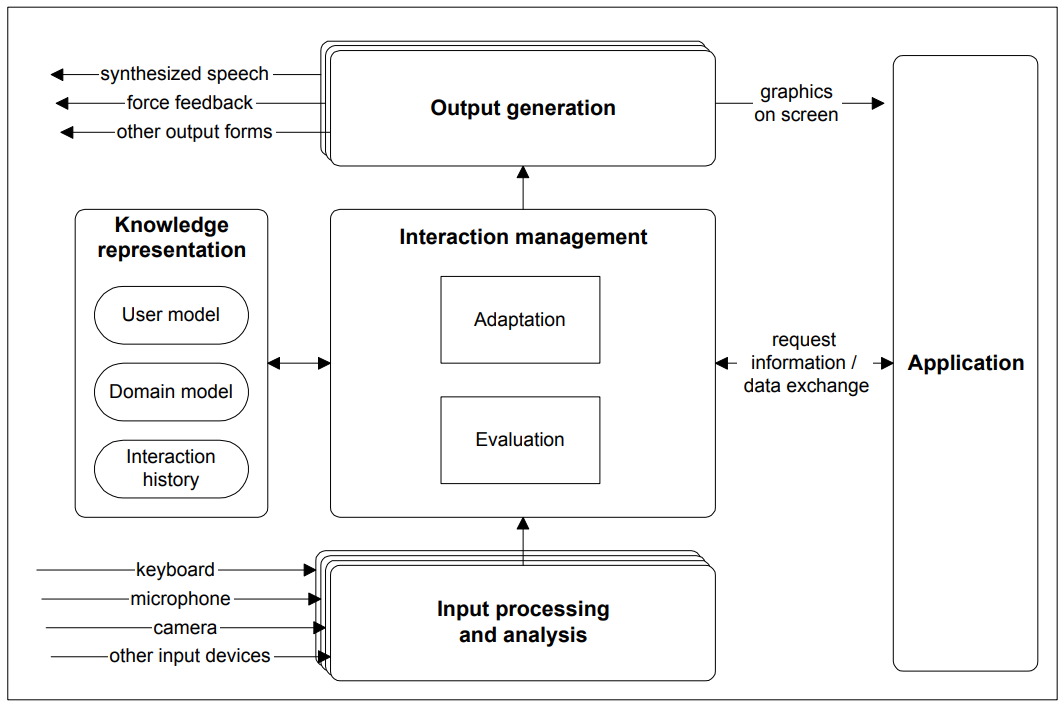
\includegraphics[scale=0.5]{images/iui_arch.png}}
\scnaddlevel{1}
    \scnrelfrom{источник}{Ehlert.P.IntellUserInterfIAS-2003art}
\scnaddlevel{-1}}

\scnhaselement{интеллектуальные технологии ввода}
\scnhaselement{моделирование пользователя}
\scnhaselement{модель пользователя}
\scnhaselement{адаптация к пользователю}
\scnhaselement{генерация пояснений}

\scnheader{моделирование пользователя}
\scnexplanation{Моделирование пользоваетля охватывает методы, которые позволяют системе поддерживать или делать выводы о пользователе на основе полученного ввода}
\lscnsource{Quote2.Ehlert.P.IntellUserInterfIAS-2003art.p4}

\scnheader{генерация пояснений}
\scnexplanation{Генерация пояснений охватывает все методы, которые позволяют системе объяснять свои результаты пользователю, например, речевой вывод, агенты интеллектуального интерфейса, тактильную обратную связь в среде виртуальной реальности.}
\lscnsource{Quote4.Ehlert.P.IntellUserInterfIAS-2003art.p4}

\scnheader{модель пользователя}
\scnexplanation{Для достижения персонализации IUI часто включают представление пользователя. Эти пользовательские модели регистрируют данные о поведении, знаниях и способностях пользователя. Новые знания о пользователе могут быть получены на основе истории ввода и взаимодействия пользователя с системой.}
\lscnsource{Quote5.Ehlert.P.IntellUserInterfIAS-2003art.p4}

\scnheader{адаптация к пользователю}
\scnexplanation{Адаптация к пользователю включает в себя все методы, которые позволяют адаптировать общение между человеком и машиной к разным пользователям и разным ситуациям, например, машинное обучение или понимание контекста.}
\lscnsource{Quote3.Ehlert.P.IntellUserInterfIAS-2003art.p4}

\scnheader{интеллектуальные технологии ввода}
\scnexplanation{Интеллектуальная технология ввода использует инновационные методы для получения ввода от пользователя. Эти методы включают в себя естественный язык, отслеживание и распознавание жестов, выражение лица распознавание и отслеживание взгляда среди прочего;}
\lscnsource{Quote1.Ehlert.P.IntellUserInterfIAS-2003art.p4}
\scnsuperset{речевой ввод}
\scnsuperset{естественно-языковой ввод}
\scnsuperset{жестовый ввод}
\scnsuperset{мимический ввод}

\scnheader{мимический ввод}
\scnsuperset{распознование лиц}
\scnaddlevel{1}
    \scnsuperset{распознование выражений лиц}
    \scnsuperset{отслеживание взгляда}
    \scnsuperset{чтение по губам}
\scnaddlevel{-1}

\scnheader{отслеживание взгляда}
\scnexplanation{Люди используют свои глаза с очень небольшим сознательным усилием. Большую часть времени мы автоматически смотрим на объект, над которым работаем. Чтобы четко видеть объект, необходимо переместить глаза так, чтобы объект оказался в центральной ямке, небольшой области в центре сетчатки. Ямка покрывает примерно один градус зрительной дуги. Из-за этого положение глаз человека обеспечивает довольно хорошую индикацию (с точностью до одного градуса ширины центральной ямки) точки фокусировки внимания человека на дисплее.}
\lscnsource{Quote3.Ehlert.P.IntellUserInterfIAS-2003.p18}

\scnheader{чтение по губам}
\scnexplanation{Проблема с распознаванием речи на основе акустического сигнала заключается в том, что оно очень плохо работает при большом количестве шума. Причина этого в том, что очень трудно отличить голос говорящего от других звуков. Идея чтения по губам заключается в том, что компьютер пытается определить, что кто-то говорит, просто глядя на движения губ человека, как глухой человек. Анализируя видеоизображения рта и используя геометрические признаки, такие как ширина и высота губ, можно определить наиболее вероятный звук (фонему).}
\lscnsource{Quote1.Ehlert.P.IntellUserInterfIAS-2003.p19}

\scnheader{жестовый ввод}
\scnexplanation{Люди часто используют жесты во время разговора, часто подсознательно. Наиболее часто используемые жесты связаны с речью, например, указывая на объект, о котором идет речь. Этот вид жестикуляции называется жестикуляцией. Жесты, функционирующие независимо от речи, называются автономными жестами, например язык жестов.}
\lscnsource{Quote1.Ehlert.P.IntellUserInterfIAS-2003art.p17}
\scnrelfrom{ввод}{жест}

\scnheader{жест}
\scnrelfromset{декомпозиция}{
    символический жест;
    дейктический жест;
    знаковый жест;
    пантомимический жест
}

\scnheader{символический жест}
\scnexplanation{Символические жесты имеют (единственное) вербальное и часто культурно-зависимое значение, например, знак «ОК» или язык жестов для глухих.}
\lscnsource{Quote2.Ehlert.P.IntellUserInterfIAS-2003.p17}

\scnheader{дейктический жест}
\scnexplanation{Дейктические жесты делаются путем указания или движения, чтобы привлечь внимание к какому-либо объекту или событию.}
\lscnsource{Quote3.Ehlert.P.IntellUserInterfIAS-2003.p17}

\scnheader{знаковый жест}
\scnexplanation{Знаковые жесты — это жесты, которые отображают информацию о размере, форме или ориентации объектов, пространственных отношениях и действиях, например, использование рук для обозначения размера пойманной рыбы).}
\lscnsource{Quote1.Ehlert.P.IntellUserInterfIAS-2003.p18}

\scnheader{пантомимический жест}
\scnexplanation{Пантомимические жесты состоят из манипулирования невидимым воображаемым объектом или инструментом, например, сжатие кулака и движение, обозначающее молоток).}
\lscnsource{Quote2.Ehlert.P.IntellUserInterfIAS-2003.p18}

\scnheader{естественно-языковой ввод}
\scnidtf{естественно-языковая система}
\scnrelfromset{декомпозиция}{
    распознавание речи;
    понимание языка;
    управление диалогом;
    запрос к базе данных;
    генерация ответа;
    речевой вывод
}

\scnheader{распознование речи}
\scnexplanation{Распознавание речи; преобразование входного речевого высказывания в строку из слов.}
\lscnsource{Quote1.Ehlert.P.IntellUserInterfIAS-2003art.p13}

\scnheader{понимание языка}
\scnexplanation{Понимание языка; анализ строки слов (насколько это возможно) для извлечения смыслового представления распознанного высказывания.}
\lscnsource{Quote2.Ehlert.P.IntellUserInterfIAS-2003art.p13}

\scnheader{управление диалогом}
\scnexplanation{Управление диалогом; управление взаимодействием или диалогом между системой и пользователем, что включает в себя координацию других компонентов системы.}
\lscnsource{Quote3.Ehlert.P.IntellUserInterfIAS-2003art.p13}

\scnheader{запрос к базе данных}
\scnexplanation{Запрос к базе данных; получение информации, запрошенной пользователем.}
\lscnsource{Quote4.Ehlert.P.IntellUserInterfIAS-2003art.p13}

\scnheader{генерация ответа}
\scnexplanation{Генерация ответа; спецификация текста, который должен быть выходным сообщением системы.}
\lscnsource{Quote5.Ehlert.P.IntellUserInterfIAS-2003art.p13}

\scnheader{речевой вывод}
\scnexplanation{Речевой вывод; фактическая генерация выходного сообщения с использованием синтеза речи или предварительно записанных фраз.}
\lscnsource{Quote6.Ehlert.P.IntellUserInterfIAS-2003art.p13}

\scnheader{мультимодальный интерфейс}
\scnexplanation{Идея мультимодальных интерфейсов заключается в использовании нескольких входных каналов при взаимодействии человека с компьютером. Вместо того, чтобы вводить только речь или текст, система может использовать распознавание изображений, чтобы смотреть на лицо или жесты пользователя. Таким образом, информация из одного режима взаимодействия может дополнять информацию, полученную из другого режима. Мультимодальные интерфейсы пытаются интегрировать речь, письменный текст, язык тела, жесты, движения глаз или губ и другие формы общения, чтобы лучше понимать пользователя и общаться более эффективно. Конечно, выбор используемых модальностей в мультимодальных интерфейсах во многом зависит от применения системы. Когда пользователи могут выбирать из нескольких способов взаимодействия с системой, система может стать доступной для более широкого круга пользователей, например для людей с ограниченными возможностями. Кроме того, мультимодальные пользовательские интерфейсы гораздо более надежны, чем обычные интерфейсы, по крайней мере, в теории. Обработка входных данных из одной модальности может быть упрощена за счет использования информации из другой, и пользователь может выбрать модальность, которая наименее подвержена ошибкам с учетом обстоятельств.}
\lscnsource{Quote1.Ehlert.P.IntellUserInterfIAS-2003art.p20}
\scnsuperset{слияние информации}

\scnheader{слияние информации}
\scnexplanation{Основным узким местом мультимодальных интерфейсов является объединение информации, полученной от используемых модальностей, в режиме реального времени. Все мультимодальные интерфейсы нуждаются в той или иной форме координации ввода или системы слияния для синхронизации связанного ввода.}
\lscnsource{Quote2.Ehlert.P.IntellUserInterfIAS-2003art.p20}
\scnrelfromset{декомпозиция}{
    слияние на уровне особенностей\\
    \scnaddlevel{1}
        \scnexplanation{Слияние на уровне функций уместно при объединении двух связанных модальностей, таких как обработка речи и движения губ. Преимуществом слияния на уровне функций является улучшенная скорость распознавания благодаря взаимодополняемости обоих входных каналов (взаимное устранение неоднозначности). Недостаток такой тесной интеграции обработки ввода заключается в том, что система должна переобучаться при изменении одной из модальностей ввода. Кроме того, обучение системы с несколькими модальностями с одновременным вводом данных намного сложнее, чем обучение одной модальности за раз.}
        \lscnsource{Quote3.Ehlert.P.IntellUserInterfIAS-2003art.p20}
    \scnaddlevel{-1};
    слияние на уровне семантики\\
    \scnaddlevel{1}
        \scnexplanation{Слияние на семантическом уровне намного проще. У него нет преимущества прямой дополнительной информации, но систему слияния на семантическом уровне гораздо проще создавать и расширять. Например, система может использовать несколько готовых методов распознавания, а новые модальности могут быть легко добавлены позже. Интеграция на семантическом уровне обычно выполняется либо путем объединения существующих данных, либо путем поиска отсутствующих данных. Последняя называется интеграцией на основе фреймов, когда системы пытаются заполнить недостающие слоты данных.}
        \lscnsource{Quote1.Ehlert.P.IntellUserInterfIAS-2003art.p20-21}
    \scnaddlevel{-1}
}

~\\
\scnauthorcomment{/* Далее идёт описание ранее неописанных компонентов интерфейса. */}
\scnheader{компонент ввода данных} 

...

    \scnsuperset{поле автозаполнения}
    \scnaddlevel{1}
        \scnidtf{autosuggest-field}
    \scnaddlevel{-1}
    
    \scnsuperset{строка навигатора}
    \scnaddlevel{1}
        \scnidtf{breadcrumb-bar}
        \scnidtf{панель навигации}
    \scnaddlevel{-1}
    
    \scnsuperset{управляющий элемент выбора даты в календаре}
    \scnaddlevel{1}
        \scnidtf{calendar-date-field}
    \scnaddlevel{-1}
    
    \scnsuperset{средство выбора цвета}
    \scnaddlevel{1}
        \scnidtf{color-palette}
        \scnidtf{палитра}
    \scnaddlevel{-1}
    
    \scnsuperset{поле со списком}
    \scnaddlevel{1}
        \scnidtf{list-field}
    \scnaddlevel{-1}
    
    \scnsuperset{ссылки на содержимое в текстовых элементах управления}
    \scnaddlevel{1}
        \scnidtf{content-link}
    \scnaddlevel{-1}
    
    \scnsuperset{управляющий элемент выбора даты}
    \scnaddlevel{1}
        \scnidtf{date-choice}
    \scnaddlevel{-1}
    
     \scnsuperset{форма}
     \scnaddlevel{1}
        \scnidtf{form}
     \scnaddlevel{-1}
     
     \scnsuperset{элемент управления рукописным вводом}
     \scnaddlevel{1}
        \scnidtf{handwriting-element}
     \scnaddlevel{-1}

\scnheader{поле автозаполнения}
\scnexplanation{Используйте AutoSuggestBox, чтобы предоставить список предложений, из которых пользователь по мере ввода текста может выбрать нужное.}
\scnaddlevel{1}
    \scneq{Quote1.Microsoft.WindowsDA-2011el}
\scnaddlevel{-1}

\scnheader{строка навигатора}
\scndefinition{Панель навигации предоставляет прямой путь к страницам или папкам в текущее расположение. Он часто используется для ситуаций, когда путь навигации пользователя (в файловой системе или системе меню) должен быть постоянно видимым, и пользователю может потребоваться вернуться к предыдущему расположению.}
\scnaddlevel{1}
    \scneq{Quote2.Microsoft.WindowsDA-2011el}
\scnaddlevel{-1}

\scnheader{управляющий элемент выбора даты в календаре}
\scndefinition{Управляющий элемент выбора даты в календаре — это раскрывающийся элемент управления, оптимизированный для выбора отдельной даты в представлении календаря, когда важна контекстная информация, например день недели или заполненность календаря. Вы можете изменить календарь таким образом, чтобы обеспечить дополнительный контекст или ограничить доступные даты.}
\scnaddlevel{1}
    \scneq{Quote3.Microsoft.WindowsDA-2011el}
\scnaddlevel{-1}

\scnheader{средство выбора цвета}
\scndefinition{Палитра используется для просмотра и выбора цвета. По умолчанию он позволяет пользователю перемещаться по цветам в цветовом спектре или указывать цвет в текстовых полях.}
\scnaddlevel{1}
    \scneq{Quote5.Microsoft.WindowsDA-2011el}
\scnaddlevel{-1}

\scnheader{поле со списком}
\scndefinition{Поле со списком (также известное как раскрывающийся список) позволяет представить список элементов, из которых пользователь может выбирать. Сначала поле со списком представлено в компактном состоянии, а затем развертывается для отображения списка элементов, доступных для выбора.}
\scnaddlevel{1}
    \scneq{Quote6.Microsoft.WindowsDA-2011el}
\scnaddlevel{-1}

\scnheader{ссылки на содержимое в текстовых элементах управления}
\scndefinition{Ссылки на содержимое позволяют вставлять в текстовые элементы управления форматированные данные. Благодаря этому пользователь может находить и использовать больше информации о людях и местах, не покидая вашего приложения.}
\scnaddlevel{1}
    \scneq{Quote10.Microsoft.WindowsDA-2011el}
\scnaddlevel{-1}

\scnheader{управляющий элемент выбора даты}
\scndefinition{Элемент выбора даты — это стандартизованный способ, позволяющий пользователям выбирать локализованное значение даты с помощью сенсорного ввода, мыши или клавиатуры.}
\scnaddlevel{1}
    \scneq{Quote11.Microsoft.WindowsDA-2011el}
\scnaddlevel{-1}

\scnheader{форма}
\scndefinition{Форма — это группа элементов управления, которые собирают данные пользователей и отправляют их. Формы обычно используются для страниц параметров, опросов, создания учетных записей и многого другого.}
\scnaddlevel{1}
    \scneq{Quote15.Microsoft.WindowsDA-2011el}
\scnaddlevel{-1}

\scnheader{элемент управления рукописным вводом}
\scndefinition{Элемент управления рукописным вводом позволяет включить в приложении базовые функции рукописного ввода}
\scnaddlevel{1}
    \scneq{Quote17.Microsoft.WindowsDA-2011el}
\scnaddlevel{-1}

\scnheader{интерактивный компонент пользовательского интерфейса}

    \scnsuperset{контекстное меню}
    \scnaddlevel{1}
        \scnidtf{раскрывающееся меню}
        \scnidtf{context-menu}
    \scnaddlevel{-1}
    
    \scnsuperset{панель команд}
    \scnaddlevel{1}
        \scnidtf{command-panel}
    \scnaddlevel{-1}
    
    \scnsuperset{карточка контакта}
    \scnaddlevel{1}
        \scnidtf{contact-card}
    \scnaddlevel{-1}
    
    \scnsuperset{диалоговые элементы управления}
    \scnaddlevel{1}
        \scnidtf{dialogue-element}
    \scnaddlevel{-1}
    
    \scnsuperset{расширитель}
    \scnaddlevel{1}
        \scnidtf{expander}
    \scnaddlevel{-1}
    
    \scnsuperset{представление пролистывания}
    \scnaddlevel{1}
        \scnidtf{scroller}
    \scnaddlevel{-1}
    
    \scnsuperset{всплывающе элементы}
    \scnaddlevel{1}
        \scnidtf{pop-up}
    \scnaddlevel{-1}
    
    \scnsuperset{представления списка и сетки}
    \scnaddlevel{1}
        \scnidtf{grid}
    \scnaddlevel{-1}
    
    \scnsuperset{гиперссылка}
    \scnaddlevel{1}
        \scnidtf{hyperlink}
    \scnaddlevel{-1}
    
    \scnsuperset{отображение карт}
    \scnaddlevel{1}
        \scnidtf{map-element}
    \scnaddlevel{-1}


\scnheader{контекстное меню}
\scndefinition{Всплывающие элементы меню используются в сценариях меню и контекстного меню для отображения списка команд или параметров, запрашиваемых пользователем.}
\scnaddlevel{1}
    \scneq{Quote18.Microsoft.WindowsDA-2011el}
\scnaddlevel{-1}

\scnheader{панель команд}
\scndefinition{Панели команд предоставляют пользователям удобный доступ к самым распространенным задачам приложения. Панели команд могут предоставлять доступ к командам приложения или страниц, работая с любым шаблоном навигации.}
\scnaddlevel{1}
    \scneq{Quote7.Microsoft.WindowsDA-2011el}
\scnaddlevel{-1}

\scnheader{карточка контакта}
\scndefinition{Карта контакта отображает контактные данные, такие как имя, номер телефона и адрес контакта. Карточка контакта также позволяет пользователю редактировать контактные данные. Можно выбрать, какую карточку следует отобразить: компактную карточку контакта или полную карточку контакта, которая содержит дополнительные сведения.}
\scnaddlevel{1}
    \scneq{Quote8.Microsoft.WindowsDA-2011el}
\scnaddlevel{-1}

\scnheader{диаологовые элемента управления}
\scndefinition{Диалоговые элементы управления — это модальные наложения пользовательского интерфейса, которые предоставляют контекстную информацию о приложении. Они блокируют взаимодействие с окном приложения, пока пользователь явно их не закроет. Они часто требуют от пользователя совершения каких-либо действий.}
\scnaddlevel{1}
    \scneq{Quote9.Microsoft.WindowsDA-2011el}
\scnaddlevel{-1}

\scnheader{расширитель}
\scndefinition{Элемент управления "Расширитель" позволяет отображать или скрывать менее важное содержимое, связанное с частью основного содержимого, которое всегда отображается. Элементы, содержащиеся в заголовке , всегда видны. Пользователь может развернуть и свернуть область содержимого , в которой отображается дополнительное содержимое, взаимодействуя с заголовком. Когда область содержимого развернута, она отправляет другие элементы пользовательского интерфейса из пути; он не накладывает другой пользовательский интерфейс. Может увеличиваться вверх или вниз.}
\scnaddlevel{1}
    \scneq{Quote12.Microsoft.WindowsDA-2011el}
\scnaddlevel{-1}

\scnheader{представление пролистывания}
\scndefinition{Используйте представление пролистывания для просмотра изображений или других элементов в коллекции, например фотографий в альбоме или элементов на странице описания продукта.}
\scnaddlevel{1}
    \scneq{Quote13.Microsoft.WindowsDA-2011el}
\scnaddlevel{-1}

\scnheader{всплывающий элемент}
\scndefinition{Всплывающий элемент — это контейнер с возможностью исчезновения, который отображает в качестве содержимого произвольный пользовательский интерфейс. Всплывающие элементы могут содержать другие вложенные всплывающие элементы или контекстные меню.}
\scnaddlevel{1}
    \scneq{Quote14.Microsoft.WindowsDA-2011el}
\scnaddlevel{-1}

\scnheader{гиперссылка}
\scndefinition{Гиперссылки используются для перехода в другую часть приложения, в другое приложение либо по указанному универсальному коду ресурса в отдельном приложении браузера.}
\scnaddlevel{1}
    \scneq{Quote16.Microsoft.WindowsDA-2011el}
\scnaddlevel{-1}

\scnheader{отображение карт}
\scndefinition{Карту можно показывать во всплывающем окне, называемом карточкой места, или в полнофункциональном элементе управления с картой.}
\scnaddlevel{1}
    \scneq{Quote19.Microsoft.WindowsDA-2011el}
\scnaddlevel{-1}

\end{small}
\end{SCn}

\newpage
\section{Формальная семантическая спецификация библиографических источников}
\begin{SCn}
\begin{small}

% https://oberoncore.ru/_media/library/c_pfister_component_software.pdf
\scnheader{Phister.C.ComponentSoftware-1997art}
\scnrelfrom{тип}{статья}
\scnrelfromlist{ключевой знак}{комопнент;компоненто-ориентированное программирование}

\scntext{аннотация}{Появление компонентного программного обеспечения может быть самым важным событием в индустрии программного обеспечения с момента появления языков программирования высокого уровня. Компонентное программное обеспечение сочетает в себе преимущества заказного и стандартного программного обеспечения. Это позволяет создавать решения, более приспособолены к эволюции, т. е. которые лучше масштабируются, которые легче обслуживать, которые можно расширять с течением времени и постепенно модернизировать.}

\scnrelfrom{цитата}{Quote1.Phister.C.ComponentSoftware-1997art.p3}
\scnaddlevel{1}
    \scneq{\scnfileitem{A component is a unit of composition with a contractually specified interface and explicit context dependencies only. Components can be deployed independently of each other and are subject to composition by third parties.}}
    %\scneq{\scnfileitem{Компонент — это элемент конструкции с определенным, зафиксированным в спецификации, интерфейсом и явными зависимостями от контекста. Компоненты могут распространяться независимо друг от друга и компоноваться третьей стороной.}}
\scnaddlevel{-1}

\scnrelfrom{цитата}{Quote2.Phister.C.ComponentSoftware-1997art.p3}
\scnaddlevel{1}
    \scneq{\scnfileitem{It is a fundamental requirement of component software that components may be developed and sold independently of each other, and yet can be combined by the customer.}}
    %\scneq{\scnfileitem{Фундаментальное требование к компонентному ПО состоит в том, чтобы компоненты могли разрабатываться и продаваться независимо друг от друга, и, таким образом, могли комбинироваться потребителем.}}
\scnaddlevel{-1}

\scnrelfrom{цитата}{Quote.Phister.C.ComponentSoftware-1997art.p4}
\scnaddlevel{1}
    \scneq{\scnfileitem{...component software is a composition of components, some of which may be standard components and others may be custom components.}}
    %\scneq{\scnfileitem{...компонентное программное обеспечение является конструкцией из компонентов, часть из которых могут быть серийными компонентами, а другие — изготовленными на заказ}}
\scnaddlevel{-1}

\scnrelfrom{цитата}{Quote.Phister.C.ComponentSoftware-1997art.p4-5}
\scnaddlevel{1}
    \scneq{\scnfileitem{By splitting a complex problem into simpler problems which can be solved independently, the problem becomes more manageable.}}
    %\scneq{\scnfileitem{При разбиении сложной проблемы на более простые, которые могут быть решены независимо друг от друга, проблема становится более управляемой.}}
\scnaddlevel{-1}

\scnrelfrom{цитата}{Quote1.Phister.C.ComponentSoftware-1997art.p5}
\scnaddlevel{1}
    \scneq{\scnfileitem{Components can be developed in parallel if it is clearly defined in advance what each component should provide, so that a programmer can immediately use the interface of a component currently being developed by another team member - even though its implementation doesn't exist yet.}}
    %\scneq{\scnfileitem{Компоненты могут разрабатываться параллельно, если заранее ясно определено, что каждый компонент должен предоставлять, так что программист может немедленно использовать интерфейс компонента, который разрабатывается другим сотрудником — даже если его реализация еще не существует.}}
\scnaddlevel{-1}

\scnrelfrom{цитата}{Quote2.Phister.C.ComponentSoftware-1997art.p5}
\scnaddlevel{1}
    \scneq{\scnfileitem{It may happen in a software project that someone remembers that some part of the current problem had already been solved for an earlier project. If this partial solution has the form of a separate component, it can be reused in the new project, thus saving time and cost.}}
    %\scneq{\scnfileitem{В программном проекте может случиться так, что кто-то вспомнит, что какая-либо часть текущей задачи уже была решена в предыдущем проекте. Если это частичное решение было оформлено как независимый компонент, оно может быть повторно использовано в новом проекте. При этом произойдет экономия времени и средств.}}
\scnaddlevel{-1}

\scnrelfrom{цитата}{Quote3.Phister.C.ComponentSoftware-1997art.p5}
\scnaddlevel{1}
    \scneq{\scnfileitem{They [buyers] get customized solutions quicker. They can save time by buying components on the market, and thereby it becomes less likely that the solutions are obsolete by the time they are ready for use. Component software allows to add new functionality over time, by adding new components to an already existing solution. In this way, a solution can be extended to handle new needs over time.}}
    %\scneq{\scnfileitem{Они [покупатели] могут сэкономить время за счет покупки компонентов на рынке, и тем самым снижают вероятность того, что программные решения уже устареют к моменту своей готовности. Компонентное ПО позволяет добавлять со временем новую функциональность, присоединяя новые компоненты к уже существующим решениям. Таким образов, решение может расширяться, чтобы соответствовать новым нуждам.}}
\scnaddlevel{-1}

\scnrelfrom{цитата}{Quote.Phister.C.ComponentSoftware-1997art.p7}
\scnaddlevel{1}
    \scneq{\scnfileitem{Component implementation is still a difficult engineering problem. The design of component interfaces is even more challenging. It takes well educated and experienced engineers to do it. Developing a truly reusable high-quality component cannot be achieved "in one shot"; it requires iterative improvement over a long time, and therefore is expensive.}}
    %\scneq{\scnfileitem{Компонентная реализация — все еще трудная инженерная проблема. Проектирование интерфейсов компонент даже еще более вызывающе. Это требует хорошо образованных и опытных инженеров. Разработка действительно многоразовых высококачественных компонентов не может быть совершена «одним выстрелом»; она требует итеративного долговременного совершенствования, и потому является дорогостоящей.}}
\scnaddlevel{-1}

\scnrelfrom{цитата}{Quote1.Phister.C.ComponentSoftware-1997art.p15}
\scnaddlevel{1}
    \scneq{\scnfileitem{The interface defines a standard for what component vendors have to provide and what component users can expect.}}
    %\scneq{\scnfileitem{Интерфейс определяет стандарт, которому производители компонентов обязаны следовать и которого пользователи вправе ожидать.}}
\scnaddlevel{-1}

\scnrelfrom{цитата}{Quote2.Phister.C.ComponentSoftware-1997art.p15}
\scnaddlevel{1}
    \scneq{\scnfileitem{
        \begin{scnitemize}
            \item a standard that enables dynamic loading of components (dynamic link libraries, calling conventions)
            \item a standard programming interface
            \item a protection mechanism which prevents a component from illegally modifying the state of other components
            \item a way to share data between components without copying them back and forth, and without explicit conversions to or from linear byte streams
        \end{scnitemize}
    }}
    %\scneq{\scnfileitem{
    %    \begin{scnitemize}
    %        \item стандарт, который допускает динамическую загрузку компонентов (динамически загружаемые библиотеки, соглашения вызовов)
    %        \item стандартный программный интерфейс
    %        \item механизм защиты, который предотвращает нелегальные изменения состояний одних компонентов другими
    %        \item способ разделения данных между компонентами без их копирования взад-вперед и без явных преобразований в линейные потоки байт
    %    \end{scnitemize}
    %}}
\scnaddlevel{-1}

\scnrelfrom{цитата}{Quote.Phister.C.ComponentSoftware-1997art.p16}
\scnaddlevel{1}
    \scneq{\scnfileitem{While the syntax of an interface can be defined easily, clear semantics are elusive. Usually there is just an informal text describing what the interface means. Formal and semi-formal specification methods can help to make interfaces less ambiguous.}}
    %\scneq{\scnfileitem{В то время как синтаксис интерфейса может быть задан очень легко, ясная семантика трудноуловима. Обычно имеется простой неформальный текст, который описывает, что из себя представляет некоторый интерфейс. Формальные и полуформальные методы специфицирования могут помочь сделать интерфейсы менее противоречивыми.}}
\scnaddlevel{-1}

\scnrelfrom{цитата}{Quote1.Phister.C.ComponentSoftware-1997art.p17}
\scnaddlevel{1}
    \scneq{\scnfileitem{...every component is required to interact with other components through their interfaces exclusively; this is a kind of universal contract, i.e., a law.}}
    %\scneq{\scnfileitem{...каждому компоненту нужно взаимодействовать с другими компонентами исключительно через их интерфейсы; это разновидность контракта, иначе говоря, закон для программиста.}}
\scnaddlevel{-1}

\scnrelfrom{цитата}{Quote2.Phister.C.ComponentSoftware-1997art.p17}
\scnaddlevel{1}
    \scneq{\scnfileitem{An interface which defines too many inessential details will cause programmers to use them and to rely on their availability. This makes it impossible to change these details later, even though it may become strongly desirable to do so. Giving too many details is especially enticing if there already exists some complex but undocumented code, which is to be turned into a component.}}
    %\scneq{\scnfileitem{Интерфейс, который задает слишком много несущественных деталей, заставит программистов использовать их и допускать их истинность. Становится невозможным изменить эти детали позже, даже если это действительно потребуется. Особенно заманчиво приводить много деталей, когда уже существует сложный и недокументированный код, который должен быть включен в компонент.}}
\scnaddlevel{-1}

\scnrelfrom{цитата}{Quote.Phister.C.ComponentSoftware-1997art.p18}
\scnaddlevel{1}
    \scneq{\scnfileitem{An object model defines the necessary rules to make components compatible on a binary level, such that components can interact on a particular machine even if they have been developed independently.}}
    %\scneq{\scnfileitem{Объектная модель определяет необходимые правила совместимости компонентов на уровне двоичного [машинного] кода, так что компоненты могут взаимодействовать на конкретной машине, даже если они разрабатывались независимо.}}
\scnaddlevel{-1}

\scnrelfrom{цитата}{Quote.Phister.C.ComponentSoftware-1997art.p18-19}
\scnaddlevel{1}
    \scneq{\scnfileitem{ A component may use the services of another component. To achieve this, a developer only needs to know the used component's interface. Possibly, there does not even exist an actual implementation for this interface yet. An interface needs to be described in some way. A textual description of an interface is written in an interface description language (IDL). Ideally, this is just a subset of the programming language that the developer uses. However, a general object model is language-independent, and of course an IDL can only be a genuine subset of very similar programming languages.}}
    %\scneq{\scnfileitem{Компонент может пользоваться услугами другого компонента. Для этого разработчику надо всего лишь знать интерфейс используемого компонента. Возможно, для этого интерфейса пока еще даже нет реальной реализации. Интерфейс должен быть некоторым образом описан. Текстовое описание интерфейса записывается на языке описания интерфейса (IDL, interface description language). В идеале, он должен быть подмножеством того языка, который использует разработчик. Однако в целом объектная модель независима от языка, и конечно же, IDL может быть подмножеством только лишь очень похожих языков программирования.}}
\scnaddlevel{-1}

\scnrelfrom{цитата}{Quote1.Phister.C.ComponentSoftware-1997art.p19}
\scnaddlevel{1}
    \scneq{\scnfileitem{An IDL description provides information about an object's interface to the developer. If possible, a compiler should use the same information to check whether the interface is used correctly. For this purpose, there often exists a binary format for interface descriptions in addition to the textual IDL format. The available collection of such binary descriptions is called the interface repository. It may just consist of a collection of so-called symbol files, or it may be stored in some kind of database.}}
    %\scneq{\scnfileitem{IDL-описание предоставляет разработчику информацию об интерфейсе объекта. Если возможно, компилятор должен использовать такую информацию для проверки того, корректно ли используется интерфейс. В этих целях часто существует двоичный формат для описание интерфейсов, в дополнение к текстовому IDL-формату. Доступный набор таких двоичных описаний называется репозиторием интерфейсов. Он может состоять просто из набора так называемых символьных файлов, или он может храниться в базе данных какого-либо рода.}}
\scnaddlevel{-1}

\scnrelfrom{цитата}{Quote2.Phister.C.ComponentSoftware-1997art.p19}
\scnaddlevel{1}
    \scneq{\scnfileitem{When a component is compiled, the compiler needs to create a file containing the generated code. The format of such a file must be suitable for run-time loading, i.e., it must be a dynamic link library.}}
    %\scneq{\scnfileitem{Когда компонент компилируется, компилятор должен создать файл, который содержит сгенерированный код. Формат такого файла должен подходить для загрузки во время выполнения, то есть, он должен быть динамически загружаемой библиотекой.}}
\scnaddlevel{-1}

\scnrelfrom{цитата}{Quote3.Phister.C.ComponentSoftware-1997art.p19}
\scnaddlevel{1}
    \scneq{\scnfileitem{At run-time, when a component for the first time needs the services of another component, this component is loaded. The loader first locates the code file of the component. Locating the code file may be straight-forward, e.g., the name of a component may directly determine the file system path to its code file. Alternatively, a configuration database may be consulted to determine the correct location of a suitable code file. This indirect approach is more flexible, but is more demanding in terms of system administration. The collection of code files or the corresponding database is called an implementation repository.}}
    %\scneq{\scnfileitem{Во время выполнения, когда компоненту первый раз потребовались услуги другого компонента, тот компонент загружается. Загрузчик сначала находит кодовый файл для компонента. Расположение кодового файла может быть очевидным, например, имя компонента может напрямую определять путь к его кодовому файлу в файловой системе. Другой вариант - текущее положение кодового файла может запрашиваться из конфигурационной базы данных. Косвенный подход более гибок, но более требователен в плане системного администрирования. Набор кодовых файлов или соответствующая база данных называются репозиторием реализации.}}
\scnaddlevel{-1}

\scnrelfrom{цитата}{Quote4.Phister.C.ComponentSoftware-1997art.p19}
\scnaddlevel{1}
    \scneq{\scnfileitem{When the loader has successfully located a component and loaded its code into memory, it can check whether the loaded code really implements the interface that was requested, and whether the versions of the loaded component and its client are compatible. This check is of fundamental importance, because it is not acceptable that a version conflict leads to a crash some time later, leaving the user without clue as to the source of the problem. Some object models provide no adequate versioning mechanism and shift the burden of consistency checking partially or completely to the client component.}}
    %\scneq{\scnfileitem{Когда загрузчик успешно нашел компонент и загрузил его код в память, он может проверить, действительно ли загруженный код реализует запрошенный интерфейс, и совместимы ли версии загруженного компонента и его клиента. Такая проверка — насущная необходимость, поскольку нельзя допустить, чтобы кофликт версий привел некоторое время спустя к краху, и при этом пользователь мог бы только догадываться о причине проблемы. Некоторые объектные модели не предоставляют адекватного механизма контроля версий и перекладывают бремя проверки соответствия частично и полностью на клиентский компонент.}}
\scnaddlevel{-1}

\scnrelfrom{цитата}{Quote5.Phister.C.ComponentSoftware-1997art.p19}
\scnaddlevel{1}
    \scneq{\scnfileitem{Once a component's code has been loaded and checked, instances of its classes can be created. For this purpose, the object model needs to define an allocation mechanism for objects. Some object models suggest an indirect approach to allocation, in order to gain additional flexibility. In particular, an object may be created by another object, a so-called factory object. A factory object may decide on its own how to allocate or how to initialize objects.}}
    %\scneq{\scnfileitem{Как только код компонента загружен и проверен, могут быть созданы экземпляры его классов. Для этих целей объектная модель должна обладать механизмом размещения объектов. Некоторые объектные модели предлагают косвенный подход к размещению, чтобы дать дополнительную гибкость. В частности, объект может создаваться другим объектом, так называемой фабрикой. Объект-фабрика может сам решать, как размещать и как инициализировать объекты.}}
\scnaddlevel{-1}

\scnrelfrom{цитата}{Quote6.Phister.C.ComponentSoftware-1997art.p19}
\scnaddlevel{1}
    \scneq{\scnfileitem{When an object thus finally has been created and made accessible to others, its methods can be called. A method call is a procedure call performed indirectly via an object, so that different objects can lead to different code being called. Typically, an object contains a pointer to a table of procedure pointers. Each element of the table corresponds to one method of the object. A method call then simply becomes an indirect procedure call via the object's method table. Usually the calling conventions of the underlying operating system are used for these procedure calls.}}
    %\scneq{\scnfileitem{После того, как объект был создан и стал доступен для других, можно вызывать его методы. Вызов метода — это вызов процедуры, который выполняется не напрямую, а через объект, так что различные объекты могут приводить к вызову различного кода. Обычно объект содержит указатель на таблицу указателей на процедуры. Каждый элемент этой таблицы соответствует одному методу объекта. Поэтому вызов метода - всего лишь непрямой вызов процедуры через таблицу методов объекта. Обычно для этих вызовов используются соглашения вызовов базовой операционной системы.}}
\scnaddlevel{-1}

\scnrelfrom{цитата}{Quote1.Phister.C.ComponentSoftware-1997art.p20}
\scnaddlevel{1}
    \scneq{\scnfileitem{ Polymorphism is one of the fundamental properties of any object-oriented or component-oriented system. In a program, some interface supported by an object may be known at compile-time. This is called its static type. But an object may reveal additional capabilities, i.e., an extended interface, at run-time. Depending on the object's dynamic type, these capabilities may differ. This is called polymorphism ("many shapes"). An object model needs to provide a means to gain access to these optional capabilities if and only if they are available. An object-oriented programming language defines language constructs such as type extension (also known as subtyping or interface inheritance), type tests, or type guards (i.e., safe type casts) for this purpose. The object model must provide similar functionality. Without polymorphism, a system would not be extensible.}}
    %\scneq{\scnfileitem{Полиморфизм — одно из главных качеств любой объектно-ориентированной или компонентно-ориентированной системы. Некотрый интерфейс, поддерживаемый объектом, может быть известен во время компиляции. Он называется его статическим типом. Но объект может приобретать дополнительные возможности, то есть, расширять свой интерфейс, во время выполнения. В зависимости от динамического типа объекта эти возможности могут отличаться. Это называется полиморфизмом («много форм»). Объектная модель должна обеспечить средства, с помощью которых можно получить доступ к таким дополнительным возможностям, если и только если они доступны. Объектно-ориентированный язык программирования в этих целях задает языковые конструкции, такие как расширение типа (также извествное как субтипизация или наследование интерфейса), проверки типа или охрана типа (то есть, безопасные преобразования между типами). Объектная модель может предоставлять похожую функциональность. Без полифморфизма система не может быть расширяемой.}}
\scnaddlevel{-1}

\scnrelfrom{цитата}{Quote2.Phister.C.ComponentSoftware-1997art.p20}
\scnaddlevel{1}
    \scneq{\scnfileitem{When an object is no longer used, i.e., when it is no longer being referenced from the outside, it must be deallocated to free the memory that it occupies. In a component world, the objects that a component makes accessible to the outside may become referenced by any number of other objects that it doesn't even know about. There must be rules that establish who must deallocate a given object, and when. For example, the object that releases the last remaining reference to another object could deallocate it. To determine whether an object owns the last reference to another one, a mechanism is needed that helps tracking references, e.g., a reference count in each object which counts the number of currently existing references to it. When the count goes down to zero, the object's memory can be freed. Correct usage by all components is critical for such rules to work. In a closed application, incorrect memory management is one of the most expensive sources of errors; but at least you know who to blame if the application crashes. In an open component world, one malfunctioning component can cause others to crash, which makes it difficult to pinpoint the culpable vendor. Thus memory management in a component software environment is a fundamentally more critical issue than for monolithic software. Ideally, the rules and mechanisms defined by an object model should be sufficiently simple, complete and clear that they can be automated; i.e., it should be possible to relieve the developer from manual deallocation, by providing an automatic garbage collector. Automatic garbage collection in an open world is no luxury, it is a necessity.}}
    %\scneq{\scnfileitem{Если объект больше не используется, то есть, на него больше нет внешних ссылок, он должен быть уничтожен, чтобы освободилась занимаемая им память. В компонентных системах на объект, который компонент предоставляет вовне, ссылаются какие-либо другие объекты, о которых сам объект ничего не знает. Поэтому должны существовать правила, которые указывают, кто и когда должен уничтожить данный объект. Например, это может сделать другой объект, у которого осталась последняя ссылка на данный. Для определения того момента, когда ссылка на объект стала последней, необходим механизм трассировки ссылок, например, счетчик ссылок в каждом объекте, который подсчитывает количество текущих ссылок на него. Когда количество становится равным нулю, память объекта может быть освобождена. Для того, чтобы такие правила работали, критически важно их правильное использование всеми компонентами. В замкнутых приложениях неправильная работа с памятью является самым главным источником ошибок; но вы, по крайней мере, знаете, кто виноват в произошедшем сбое. В открытых компонентных системах один неправильно работающий компонент может привести к краху всю систему, при этом сложно определить виновного производителя. Поэтому управление памятью в компонентной программной среде является принципиально более важным вопросом, чем в монолитном ПО. В идеале правила и механизмы, вводимые объектной моделью, должны быть достаточно простыми, полными и ясными, чтобы их можно было автоматизировать, то есть, освободить разработчика от ручной работы, предоставив автоматический сборщик мусора. Автоматический сборщик мусора в открытых системах - это не роскошь, а необходимость.}}
\scnaddlevel{-1}

\scnrelfrom{цитата}{Quote3.Phister.C.ComponentSoftware-1997art.p20}
\scnaddlevel{1}
    \scneq{\scnfileitem{An object model that supports distributed objects must define a message format, which describes the byte streams produced by a remote method call. The caller of a method is called the client, the callee is called the server. In the most general scenario, the server object is implemented on another machine than the client. From a developer's perspective, the client can directly call a server object's methods. In reality, the client only interacts with a proxy object, which is a local representation of the true object implementation on the remote server machine. In most implementations, a proxy, as well as its server-side counterpart, can be generated automatically out of the object's interface.}}
    %\scneq{\scnfileitem{Объектная модель, которая поддерживает распределенные объекты, должна определять формат сообщений, который описывает потоки байт, порождаемые удаленным вызовом методов. Того, кто вызывает метод, называют клиентом, того, чей метод вызывают, — сервером. По самому общему сценарию серверный объект и клиент выполняются на разных машинах. С точки зрения разработчика клиент может напрямую вызывать методы серверного объекта. В реальности клиент взаимодействует всего лишь с прокси объектом, который является локальным представителем настоящего объекта, работающего на удаленной серверной машине. В большинстве реализаций прокси-объект, также как и его аналог на стороне сервера, могут генерироваться автоматически из интерфейса объекта.}}
\scnaddlevel{-1}



% https://books.google.by/books?id=U896iwmtiagC
\scnheader{Szyperski.C.CompSoftBOOP-2002book}
\scnrelfrom{тип}{книга}
\scnrelfromlist{ключевой знак}{компонент;компонентное проектирование;компоненто-ориентированное программирование}
\scntext{аннотация}{Книга посвящена посвящена компонентному проектированию, как способу повторно использовать уже разработанное программное обеспечение.}

\scnrelfrom{цитата}{Quote.Szyperski.C.CompSoftBOOP-2002book.p10}
\scnaddlevel{1}
    \scneq{\scnfileitem{A software component is what is actually deployed – as an isolatable part of a system – in a component-based approach. Contrary to frequent claims, objects are almost never sold, bought, or deployed.}}
    %\scneq{\scnfileitem{Программный компонент -- то, что непосредственно разворачивается -- как изолируемая часть системы -- в компонентно-ориентированном подходе. Вопреки частым утверждениям, объекты почти никогда не продаются, не покупаются и не разворачиваются.}}
    \scnrelfromset{сравнение}{компонентное программное обеспечение;объектно-ориентированное программное обеспечение}
\scnaddlevel{-1}

\scnrelfrom{цитата}{Quote1.Szyperski.C.CompSoftBOOP-2002book.p11}
\scnaddlevel{1}
    \scneq{\scnfileitem{...a component could just as well use some totally different implementation technology, such as pure functions or assembly language, and look not at all object-oriented from the inside.}}
    %\scneq{\scnfileitem{...при разработке компонента также может быть использована совсем иная технология, такая как чистые функции или язык ассемблера, которые не имеют ничего общего с объектно-ориентированностью изнутри.}}
    \scnrelfromset{сравнение}{компонентное программное обеспечение;объектно-ориентированное программное обеспечение}
\scnaddlevel{-1}

\scnrelfrom{цитата}{Quote2.Szyperski.C.CompSoftBOOP-2002book.p11}
\scnaddlevel{1}
    \scneq{\scnfileitem{The definition [of object] does not include notions of independence or late composition.}}
    %\scneq{\scnfileitem{Определение [объекта] не включает в себя независимости или компонуемости.}}
    \scnrelfromset{сравнение}{компонентное программное обеспечение;объектно-ориентированное программное обеспечение}
\scnaddlevel{-1}

\scnrelfrom{цитата}{Quote1.Szyperski.C.CompSoftBOOP-2002book.p36}
\scnaddlevel{1}
    \scneq{\scnfileitem{For a component to be independently deployable, it needs to be well separated from its environment and other components.}}
    %\scneq{\scnfileitem{Для того, чтобы компонент можно было развернуть независимо, он должен быть отделён от своего окружения и других компонентов.}}
\scnaddlevel{-1}

\scnrelfrom{цитата}{Quote2.Szyperski.C.CompSoftBOOP-2002book.p36}
\scnaddlevel{1}
    \scneq{\scnfileitem{...it [component] needs to come with clear specifications of what it requires and provides. In other words, a component needs to encapsulate its implementation and interact with its environment by means of well-defined interfaces.}}
    %\scneq{\scnfileitem{...он [компонент] должен поставляться с чёткой спецификацией того, что он требует и предоставляет. Другими словами, компонент должен скрывать свою имплементацию и взаимодействовать с окружением при помощи чётко определённых интерфейсов.}}
\scnaddlevel{-1}

\scnrelfrom{цитата}{Quote3.Szyperski.C.CompSoftBOOP-2002book.p36}
\scnaddlevel{1}
    \scneq{\scnfileitem{...a component should not have any (externally) observable state.}}
    %\scneq{\scnfileitem{...компонент не должен иметь наблюдаемого (извне) состояния.}}
\scnaddlevel{-1}

\scnrelfrom{цитата}{Quote4.Szyperski.C.CompSoftBOOP-2002book.p36}
\scnaddlevel{1}
    \scneq{\scnfileitem{...it makes little sense to have multiple copies [of a component] in the same operating system process as these would be mutually indistinguishable anyway. In other words, in any given process (or other loading context), there will be at most one copy of a particular component.}}
    %\scneq{\scnfileitem{...не имеет смысла иметь несколько копий [компонента] в одной и той же операционной системе, поскольку они в любом случае будут фактически неотличимы. Другими словами, в любом процессе (или ином контексте), не должно быть более одной копии конкретного компонента.}}
\scnaddlevel{-1}

\scnheader{USGenServAdm.2.101.Definitions-reg}\\
\scnrelfrom{тип}{закон}\\
\scnrelfrom{цитата}{Quote.USGenServAdm.2.101.Definitions-reg}
\scnaddlevel{1}
    \scneq{\scnfileitem{
    Commercially available off-the-shelf (COTS) item means any item of supply (including construction material) that is
    \begin{scnitemize}
        \item A commercial product (as defined in paragraph (1) of the definition of “commercial product” in this section);
        \item Sold in substantial quantities in the commercial marketplace; and
        \item Offered to the Government [customer], under a contract or subcontract at any tier, without modification, in the same form in which it is sold in the commercial marketplace; 
    \end{scnitemize}
    }}
\scnaddlevel{-1}

\scnheader{Khan.A.PerspecStudyISFCBD-2015art}
\scnrelfrom{тип}{статья}
\scntext{аннотация}{Nowadays, researchers envisage an Intelligent ComponentOriented Software Development methodology which is an amalgam of the two approaches resulting in more flexible, reusable and customizable agent components. This helps in pushing forward the development timelines and quality expectations to newer heights. In this paper we mainly analyzed various states of art intelligent component-oriented software development techniques and studied the research gap in the component selection processes. Recommendations for future research direction for Intelligent Component-Oriented Software Development are also highlighted in this paper.}
% Multi-agent control, Component Based Development, Agentbased modeling, Self-adaptive systems
\scnrelfromlist{ключевой знак}{
    мультиагентные системы;
    компоненто-ориентированное проектирование;
    агенто-ориентированное проектирование;
    самоадаптирующиеся системы
}
\scnrelfrom{цитата}{Quote1.Khan.A.PerspecStudyISFCBD-2015art-p.11}
\scnaddlevel{1}
    \scneq{\scnfileitem{It is very difficult to guess how the components behave under different conditions and environments as mostly COTS software comes up as a black box with limited access.}}
\scnaddlevel{-1}
\scnrelfrom{цитата}{Quote2.Khan.A.PerspecStudyISFCBD-2015art-p.11}
\scnaddlevel{1}
    \scneq{\scnfileitem{It is also difficult to map user requirement to the component based architecture and generally there is a need for a process which fully customized the component as per the customer requirement.}}
\scnaddlevel{-1}
\scnrelfrom{цитата}{Quote.Khan.A.PerspecStudyISFCBD-2015art-p.11-12}
\scnaddlevel{1}
    \scneq{\scnfileitem{In order to developed application from components or tailor components to a new situation, efforts are required to build wrappers and the glue between components, since most of the COTS software lacks in plug and play technique and developer has to build wrappers for component integration. Further, wrappers need to be maintained as the system evolves.}}
\scnaddlevel{-1}
\scnrelfrom{цитата}{Quote1.Khan.A.PerspecStudyISFCBD-2015art-p.12}
\scnaddlevel{1}
    \scneq{\scnfileitem{Components are packaged and delivered in many different forms (example: function libraries, off-the shelf applications and frameworks).}}
\scnaddlevel{-1}
\scnrelfrom{цитата}{Quote2.Khan.A.PerspecStudyISFCBD-2015art-p.12}
\scnaddlevel{1}
    \scneq{\scnfileitem{Most component integration processes suffer from inflexibility by a lack of component evaluation schemes. This problem is often compounded by a lack of interoperability standards between component frameworks and adequate vendor support.}}
\scnaddlevel{-1}

\scnheader{Maybury.M.IntellUserInterfIntro-1998art}
\scnrelfrom{тип}{статья}
\scnrelfromlist{ключевой знак}{пользовательский интерфейс;интеллектуальный пользовательский интерфейс}
\scntext{аннотация}{В этом введении описывается потребность в интеллектуальных пользовательских интерфейсах (IUI), определяется основная терминология, используемая в этой области. После описания теоретических основ интеллектуальных пользовательских интерфейсов в этом вводном разделе описываются современное состояние дел и обобщает структуру и содержание этой коллекции, в которой рассматриваются некоторые остающиеся фундаментальные проблемы в этой области.}

\lscnquote{Quote1.Maybury.M.IntellUserInterfIntro-1998art.p2}{Intelligent user interfaces (IUIs) are human-machine interfaces that aim to improve the efficiency, effectiveness, and naturalness of human-machine interaction by representing, reasoning, and acting on models of the user, domain, task, discourse, and media (e.g., graphics, natural language, gesture). As a consequence, this interdisciplinary area draws upon research in and lies at the intersection of human-computer interaction, ergonomics, cognitive science, and artificial intelligence and its subareas (e.g., vision, speech and language processing, knowledge representation and reasoning, machine learning/knowledge discovery, planning and agentmodeling, user and discourse modeling). }

\lscnquote{Quote1.Maybury.M.IntellUserInterfIntro-1998art.p3-4}{The "intelligence" in IUIs that distinguishes them from traditional interfaces... it [IUI] includes mechanisms that perform automated media analysis, design, and interaction management... Traditional user interfaces distinguish only three models: presentation, dialog, and application. Refinements beyond these three models that are found in IUIs include explicit models of the user, discourse and domain, input analysis and output generation, and mechanisms to manage the interaction, such as fusing and interpreting imprecise, ambiguous, and/or inaccurate input, controlling the dialog progression, or tailoring presentation output to the current situation. Research so far has shown that it is possible to adapt many of the fundamental concepts developed to date in computational linguistics and discourse theory in such a way that they become useful for multimedia user interfaces as well. In particular, semantic and pragmatic concepts like communicative acts, coherence, focus, reference, discourse model, user model, implicature, anaphora, rhetorical relations, and scope ambiguity take on an extended meaning in the context of multimodal communication... artificial intelligence has much to contribute to user interfaces, including the use of knowledge representations for model-based interface development tools. Architecture of Intelligent User Interfaces application of plan generation and recognition in dialog management, the application of temporal and spatial reasoning to media coordination, the use of user models to tailor interaction, and so on.}

\scnheader{Ehlert.P.IntellUserInterfIAS-2003art}
\scnrelfrom{тип}{статья}
\scnrelfromlist{ключевой знак}{интеллектуальный пользовательский интерфейс; IUI; intelligent user interface; адаптивный интерфейс; взаимодействие человек-компьютер; модель пользователя; распознавание плана; мультимодальное взаимодействие; интеллектуальные агенты; software usability; искусственный интеллект}
\scntext{аннотация}{Этот отчет является частью исследования литературы по интеллектуальным пользовательским интерфейсам. Цель этого отчета состоит в том, чтобы представить область, объяснить концепции и предоставить глобальный обзор существующих приложений (исследований) с интеллектуальным пользовательским интерфейсом. Этот отчет предназначен для ученых-компьютерщиков или опытных пользователей компьютеров. Чтобы полностью понять
отчет, некоторые базовые знания об искусственном интеллекте могут быть полезны.}
\lscnquote{Quote1.Ehlert.P.IntellUserInterfIAS-2003art.p2}{
\begin{scnitemize}
        \item \textbf{Creating personalized systems}\\
        No two persons are the same and people have different habits, preferences, and working methods and environment. An intelligent interface that takes these differences into account can provide a personalized method of interaction. The interface knows the user and can use that knowledge in its communication with the user.
        \item \textbf{Information overflow or filtering problems}\\
        Finding the right information on your computer or on the Internet can be like looking for a needle in a haystack. Intelligent interfaces can reduce the information overload that often results from finding information in large databases or complex systems. By filtering out irrelevant information, the interface can reduce the cognitive load on the user. In addition, the IUI can propose new and useful information sources not known to the user.
        \item \textbf{Providing help on using new and complex programs}\\
        Computer systems can be very complicated to work with when you first start to use them. As you struggle to get to know and understand a new program, new software versions or updates may appear that include new functionality. Many computer users fail to keep up with these developments. Intelligent help systems can detect and correct user misconceptions, explain new concepts, and provide information to simplify tasks.
        \item \textbf{Taking over tasks from the user}\\
        An IUI can also look at what you are doing, understand and recognize your intent, and take over some of your tasks completely, allowing you to focus on other things.
        \item \textbf{Other forms of interaction}\\
        Currently, the most common interaction devices are the keyboard and the mouse. IUIresearch looks at other forms of human-computer interaction (e.g. speech or gestures). By providing multiple forms of interaction, people with a disability will be able to use computers more easily. 
    \end{scnitemize}
}
\lscnquote{Quote1.Ehlert.P.IntellUserInterfIAS-2003art.p4}{Intelligent input technology uses innovative techniques to get input from a user. These techniques include natural language, gesture tracking and recognition, facial expression recognition, and gaze tracking among others; }
\lscnquote{Quote2.Ehlert.P.IntellUserInterfIAS-2003art.p4}{User modeling covers techniques that allow a system to maintain or infer knowledge about
a user based on the received input}
\lscnquote{Quote3.Ehlert.P.IntellUserInterfIAS-2003art.p4}{User adaptivity includes all techniques that allow the communication between human and machine to be adapted to different users and different situations for example, machine learning or context awareness}
\lscnquote{Quote4.Ehlert.P.IntellUserInterfIAS-2003art.p4}{Explanation generation covers all techniques that allow a system to explain its results to a user for example, speech output, intelligent interface agents, tactile feedback in a virtual reality environment. }
\lscnquote{Quote5.Ehlert.P.IntellUserInterfIAS-2003art.p4}{To achieve personalization, IUIs often include a representation of a user. These user models log data about the userís behavior, knowledge, and abilities. New knowledge about the user can be inferred based on the input and interaction history of the user with the system.}
\lscnquote{Quote1.Ehlert.P.IntellUserInterfIAS-2003.p5}{An often-made mistake is to confuse an IUI with an intelligent system. A system exhibiting some form of intelligence is not necessarily an intelligent interface. There are many intelligent systems with very simple non-intelligent interfaces and the fact that a system has an intelligent interface does not say anything about the intelligence of the underlying system}
\lscnquote{Quote1.Ehlert.P.IntellUserInterfIAS-2003.p8}{
\begin{scnitemize}
    \item An adaptive user interface must be developed in parallel with the application. This is necessary since the designer continuously needs to focus on the system parts that need to be adapted.
    \item Do not disturb the user's interaction. It should always be possible for the user to ignore the proactive actions of the IUI. Suggest rather than act.
    \item Operate in real-time. Much of the benefit of an IUI comes from acting while the user is busy working with the system.
    \item Take advantage of the user's think time. When the user is thinking about what input to provide next, the IUI can take advantage of the available processing time, so it does not risk slowing down the userís interaction with the system.
    \item Watch what the user is doing. Take advantage of ìfreeî information implicit in user actions.
    \item Allow the user to choose his personal interaction style. Different users like different interface styles and some techniques may be distracting or confusing to some users. 
\end{scnitemize}}
\lscnquote{Quote1.Ehlert.P.IntellUserInterfIAS-2003.p9-10}{
\begin{scnitemize}
    \item An adaptive system is unpredictable and less transparent than a DM interface. If a system can adapt its response and does not give the same response twice given the same input, then the system becomes unpredictable. This will hinder the userís comprehension of the system, making it impossible for him to do a successful action twice. 
    \item Users are not in control anymore. An IUI can make decisions for the user, thus placing the user outside the control loop.
    \item IUIs often make mistakes. Many IUI systems use trail and error to determine a userís intent or preferences. Therefore users need to give feedback to the system or even resolve the mistakes made by the system.
    \item Simulated intelligence and adaptivity increases the risk of the user thinking that computer can do things that it cannot, thus creating false expectations. Especially with anthropomorphic agents users may believe they can interact with the IUI just as with another person.
    \item Who is responsible? If a system can make decisions on its own, who is responsible for the actions: the programmer of the system, the user, or the system itself?
    \item What about the privacy and thrust of the user? What happens to the user profile that is created and maintained by an IUI? Can you guarantee that it is safe and will not be misused?
\end{scnitemize}}
\lscnquote{Quote1.Ehlert.P.IntellUserInterfIAS-2003art.p13}{Speech recognition; conversion of an input speech utterance into a string of words. }
\lscnquote{Quote2.Ehlert.P.IntellUserInterfIAS-2003art.p13}{Language understanding; analysis of the string of words (as much as possible) to extract a meaning representation for the recognized utterance.}
\lscnquote{Quote3.Ehlert.P.IntellUserInterfIAS-2003art.p13}{Dialogue management; controlling the interaction or dialogue between the system and the user, which includes coordination of other components of the system.}
\lscnquote{Quote4.Ehlert.P.IntellUserInterfIAS-2003art.p13}{Database query; retrieving the information requested by the user. }
\lscnquote{Quote5.Ehlert.P.IntellUserInterfIAS-2003art.p13}{Response generation; specification of the text that is to be the output message of the system.}
\lscnquote{Quote6.Ehlert.P.IntellUserInterfIAS-2003art.p13}{Speech output; actual generation of the output message using text-to-speech synthesis or prerecorded sentences.}
\lscnquote{Quote1.Ehlert.P.IntellUserInterfIAS-2003art.p17}{People use gestures a lot when talking, often subconsciously. The most often-used gestures are those associated with speech, for example pointing to an object that one is referring to. This kind of gesturing is called gesticulation. Gestures that function independent of speech are called autonomous gestures, for example sign language.}
\lscnquote{Quote2.Ehlert.P.IntellUserInterfIAS-2003.p17}{Symbolic gestures have a (single) verbal and often cultural dependant meaning, for example the OK sign, or sign language for deaf people.}
\lscnquote{Quote3.Ehlert.P.IntellUserInterfIAS-2003.p17}{Deictic gestures are made by pointing or motioning to direct attention to some object or
event.}
\lscnquote{Quote1.Ehlert.P.IntellUserInterfIAS-2003.p18}{Iconic gestures are gestures that display information about the size, shape or orientation of objects, spatial relations, and actions, for example using hands to indicate the size of fish that one caught).}
\lscnquote{Quote2.Ehlert.P.IntellUserInterfIAS-2003.p18}{Pantomimic gestures consist of manipulating an invisible imaginary object or tool, for example making a fist and moving to indicate a hammer).}
\lscnquote{Quote3.Ehlert.P.IntellUserInterfIAS-2003.p18}{People use their eyes with very little conscious effort. Most of the time, we automatically look at the object we are working on. To see an object clearly, it is necessary to move your eyes so that the object appears on the fovea, a small area at the center of the retina. The fovea covers approximately one degree of visual arc. Because of this, a personís eye position provides a rather good indication (to within the one-degree width of the fovea) of a personís focus point of attention on a display.}
\lscnquote{Quote1.Ehlert.P.IntellUserInterfIAS-2003.p19}{A problem with speech recognition based on an acoustic signal, is that it functions very badly when there is a lot of noise. The reason for this is that it is very hard to distinguish the speakerís voice from other sounds. With lip reading the idea is that the computer tries to determine what someone is saying just by looking at the personís lip movements, like a deaf person. By analyzing video images of the mouth and using geometric features, such as the width and height of the lips, the most probable sound (phoneme) can be determined.}
\lscnquote{Quote1.Ehlert.P.IntellUserInterfIAS-2003art.p20}{With multimodal interfaces, the idea is to use multiple input channels in human-computer interaction. Instead of only speech or text as input, the system can use image recognition to look at a userís face or gestures. This way, information from one mode of interaction can complement the information received from another mode. Multimodal interfaces try to integrate speech, written text, body language, gestures, eye or lip movements and other forms of communication in order to better understand the user and to communicate more effectively. Of course, the choice of the used modalities in multimodal interfaces depends very much on the application of the system. When users can choose from multiple modalities to interact with a system, the system has the potential to be accessible to a broader range of users, for example people with disabilities. Also, multimodal user interfaces are much more robust than normal interfaces, at least in theory. Processing input from one modality can be simplified by using information from another and the user can choose the modality that is the least error prone given the circumstances.}
\lscnquote{Quote2.Ehlert.P.IntellUserInterfIAS-2003art.p20}{The main bottleneck in multimodal interfaces is to combine the information gathered from the used modalities in real time. All multimodal interfaces need some form of input coordination or fusion system to synchronize related input.}
\lscnquote{Quote3.Ehlert.P.IntellUserInterfIAS-2003art.p20}{Feature-level fusion is appropriate when combining two related modalities, such as speech processing and lip movements. The advantage of feature-level fusion is the improved recognition rate due to the complementary nature of both input channels (mutual disambiguation). A drawback of this tight integration of input processing is that the system has to be retrained when the one of the input modalities is changed. In addition, training a system with multiple modalities using simultaneous input is much more difficult than training one modality at the time.}
\lscnquote{Quote1.Ehlert.P.IntellUserInterfIAS-2003art.p20-21}{Semantic-level fusion is much easier. It does not have the benefit of direct complementary information, but a semantic-level fusion system is much easier to create and extend. Such as system can use multiple off-the-shelf recognition techniques and new modalities can easily be added later. Semantic-level integration is usually done either through unification of existing data or by looking for missing data. The latter is called frame-based integration, where the systems tries to fill missing data slots.}
\lscnquote{Quote1.Ehlert.P.IntellUSerInterfIAS-2003.p36}{
\begin{scnitemize}
    \item Cognitive theory and empirical science underpinnings. A better understanding is required of the unique linguistic and performance characteristics of natural communication modalities (speech, gesture, gaze and facial expressions) and of how these modalities can be combined best.
    \item New multimodal interface concepts. Current research on multimodal interfaces has focused mainly on natural language processing, pen-based gestures. Additional input such as body motion and facial expressions should be studied.
    \item Multimodal language and dialogue processing. A general theory of conversational interaction is needed that deals with intent representation for non-speech modalities.
    \item Error handling techniques. Graceful error handling is still a problem in multimodal interfaces and mutual disambiguation between signals can be improved. Also the impact of a third or more modalities on the error rate should be studied, as well as performance under
    difficult (mobile) environments.
    \item Adaptive multimodal architectures. Multimodal architectures are hardly adaptive and adapting to a specific user or environment can increase the recognition of input processing, as well as provide more flexibility and ease of use for the user.
    \item Multi-device multi-user ubiquitous computing. In the future, mobile computing will become more important, so we need to look at the role of multimodal interfaces in that area. In addition, when multiple users are interacting together, for example via the Internet, interfaces need to take multiple input from remote devices into account.
    \item Multimodal research infrastructure. Supporting tools for multimodal interface research should be developed. This includes; semi-automatic simulation methods for empirical data collection and prototyping of new systems, automated tools for collecting and analyzing multimodal corpora, novel metrics for evaluating multimodal systems, and software tools that support the rapid creation of next-generation multimodal applications. 
\end{scnitemize}}

\scnheader{Microsoft.WindowsDA-2011el}
\scnrelfrom{тип}{электронный ресурс}
\scnrelfromlist{ключевой знак}{интерфейс;компоненты интерфейса}
\scntext{аннотация}{Руководство по проектированию и примеры кода пользовательского интерфейса для создания процессов взаимодействия с приложениями для Windows.}

\scntext{url}{https://docs.microsoft.com/en-US/windows/apps/design}

\scnrelfrom{цитата}{Quote1.Microsoft.WindowsDA-2011el}
\scnaddlevel{1}
    \scneq{\scnfileitem{Use an AutoSuggestBox to provide a list of suggestions for a user to select from as they type.}}
    %\scneq{\scnfileitem{Используйте AutoSuggestBox, чтобы предоставить список предложений, из которых пользователь по мере ввода текста может выбрать нужное.}}
    \scntext{url}{https://docs.microsoft.com/en-us/windows/apps/design/controls/auto-suggest-box}
\scnaddlevel{-1}

\scnrelfrom{цитата}{Quote2.Microsoft.WindowsDA-2011el}
\scnaddlevel{1}
    \scneq{\scnfileitem{A BreadcrumbBar provides the direct path of pages or folders to the current location. It is often used for situations where the user's navigation trail (in a file system or menu system) needs to be persistently visible and the user may need to go back to a previous location.}}
    %\scneq{\scnfileitem{Панель навигации предоставляет прямой путь к страницам или папкам в текущее расположение. Он часто используется для ситуаций, когда путь навигации пользователя (в файловой системе или системе меню) должен быть постоянно видимым, и пользователю может потребоваться вернуться к предыдущему расположению.}}
    \scntext{url}{https://docs.microsoft.com/en-US/windows/apps/design/controls/breadcrumbbar}
\scnaddlevel{-1}

\scnrelfrom{цитата}{Quote3.Microsoft.WindowsDA-2011el}
\scnaddlevel{1}
    \scneq{\scnfileitem{The calendar date picker is a drop down control that's optimized for picking a single date from a calendar view where contextual information like the day of the week or fullness of the calendar is important. You can modify the calendar to provide additional context or to limit available dates.}}
    %\scneq{\scnfileitem{Управляющий элемент выбора даты в календаре — это раскрывающийся элемент управления, оптимизированный для выбора отдельной даты в представлении календаря, когда важна контекстная информация, например день недели или заполненность календаря. Вы можете изменить календарь таким образом, чтобы обеспечить дополнительный контекст или ограничить доступные даты.}}
    \scntext{url}{https://docs.microsoft.com/en-US/windows/apps/design/controls/calendar-date-picker}
\scnaddlevel{-1}

\scnrelfrom{цитата}{Quote4.Microsoft.WindowsDA-2011el}
\scnaddlevel{1}
    \scneq{\scnfileitem{A calendar view lets a user view and interact with a calendar that they can navigate by month, year, or decade. A user can select a single date or a range of dates. It doesn't have a picker surface and the calendar is always visible.}}
    %\scneq{\scnfileitem{Представление календаря позволяет пользователю просматривать календарь и взаимодействовать с ним, перемещаясь по месяцам, годам и десятилетиям. Пользователь может выбрать отдельную дату или диапазон дат. Не имеет поверхности выбора, и календарь всегда виден.}}
    \scntext{url}{https://docs.microsoft.com/en-us/windows/apps/design/controls/calendar-view}
\scnaddlevel{-1}

\scnrelfrom{цитата}{Quote5.Microsoft.WindowsDA-2011el}
\scnaddlevel{1}
    \scneq{\scnfileitem{A color picker is used to browse through and select colors.}}
    %\scneq{\scnfileitem{Палитра используется для просмотра и выбора цвета.}}
    \scntext{url}{https://docs.microsoft.com/en-us/windows/apps/design/controls/color-picker}
\scnaddlevel{-1}

\scnrelfrom{цитата}{Quote6.Microsoft.WindowsDA-2011el}
\scnaddlevel{1}
    \scneq{\scnfileitem{Use a combo box (also known as a drop-down list) to present a list of items that a user can select from. A combo box starts in a compact state and expands to show a list of selectable items. A list box is similar to a combo box, but is not collapsible/does not have a compact state.}}
    %\scneq{\scnfileitem{Поле со списком (также известное как раскрывающийся список) позволяет представить список элементов, из которых пользователь может выбирать. Сначала поле со списком представлено в компактном состоянии, а затем развертывается для отображения списка элементов, доступных для выбора. Поле со списком похоже на поле со списком, но не свертывается или не имеет компактного состояния.}}
    \scntext{url}{https://docs.microsoft.com/en-us/windows/apps/design/controls/combo-box}
\scnaddlevel{-1}

\scnrelfrom{цитата}{Quote7.Microsoft.WindowsDA-2011el}
\scnaddlevel{1}
    \scneq{\scnfileitem{Command bars provide users with easy access to your app's most common tasks. Command bars can provide access to app-level or page-specific commands and can be used with any navigation pattern.}}
    %\scneq{\scnfileitem{Панели команд предоставляют пользователям удобный доступ к самым распространенным задачам приложения. Панели команд могут предоставлять доступ к командам приложения или страниц, работая с любым шаблоном навигации.}}
    \scntext{url}{https://docs.microsoft.com/en-us/windows/apps/design/controls/command-bar}
\scnaddlevel{-1}

\scnrelfrom{цитата}{Quote8.Microsoft.WindowsDA-2011el}
\scnaddlevel{1}
    \scneq{\scnfileitem{The contact card displays contact information, such as the name, phone number, and address, for a Contact. The contact card also lets the user edit contact info.}}
   % \scneq{\scnfileitem{Карта контакта отображает контактные данные, такие как имя, номер телефона и адрес контакта. Карточка контакта также позволяет пользователю редактировать контактные данные.}}
    \scntext{url}{https://docs.microsoft.com/en-us/windows/apps/design/controls/contact-card}
\scnaddlevel{-1}

\scnrelfrom{цитата}{Quote9.Microsoft.WindowsDA-2011el}
\scnaddlevel{1}
    \scneq{\scnfileitem{Dialog controls are modal UI overlays that provide contextual app information. They block interactions with the app window until being explicitly dismissed. They often request some kind of action from the user.}}
    %\scneq{\scnfileitem{Диалоговые элементы управления — это модальные наложения пользовательского интерфейса, которые предоставляют контекстную информацию о приложении. Они блокируют взаимодействие с окном приложения, пока пользователь явно их не закроет. Они часто требуют от пользователя совершения каких-либо действий.}}
    \scntext{url}{https://docs.microsoft.com/en-us/windows/apps/design/controls/dialogs-and-flyouts/dialogs}
\scnaddlevel{-1}

\scnrelfrom{цитата}{Quote10.Microsoft.WindowsDA-2011el}
\scnaddlevel{1}
    \scneq{\scnfileitem{Content links provide a way to embed rich data in your text controls, which lets a user find and use more information about a person or place without leaving the context of your app.}}
    %\scneq{\scnfileitem{Ссылки на содержимое позволяют вставлять в текстовые элементы управления форматированные данные. Благодаря этому пользователь может находить и использовать больше информации о людях и местах, не покидая вашего приложения.}}
    \scntext{url}{https://docs.microsoft.com/en-us/windows/apps/design/controls/content-links}
\scnaddlevel{-1}

\scnrelfrom{цитата}{Quote11.Microsoft.WindowsDA-2011el}
\scnaddlevel{1}
    \scneq{\scnfileitem{The date picker gives you a standardized way to let users pick a localized date value using touch, mouse, or keyboard input.}}
    %\scneq{\scnfileitem{Элемент выбора даты — это стандартизованный способ, позволяющий пользователям выбирать локализованное значение даты с помощью сенсорного ввода, мыши или клавиатуры.}}
    \scntext{url}{https://docs.microsoft.com/en-us/windows/apps/design/controls/date-picker}
\scnaddlevel{-1}

\scnrelfrom{цитата}{Quote12.Microsoft.WindowsDA-2011el}
\scnaddlevel{1}
    \scneq{\scnfileitem{The Expander control lets you show or hide less important content that's related to a piece of primary content that's always visible.}}
    %\scneq{\scnfileitem{Элемент управления "Расширитель " позволяет отображать или скрывать менее важное содержимое, связанное с частью основного содержимого, которое всегда отображается.}}
    \scntext{url}{https://docs.microsoft.com/en-us/windows/apps/design/controls/expander}
\scnaddlevel{-1}

\scnrelfrom{цитата}{Quote13.Microsoft.WindowsDA-2011el}
\scnaddlevel{1}
    \scneq{\scnfileitem{Use a flip view for browsing images or other items in a collection, such as photos in an album or items in a product details page, one item at a time.}}
    %\scneq{\scnfileitem{Используйте представление пролистывания для просмотра изображений или других элементов в коллекции, например фотографий в альбоме или элементов на странице описания продукта. Каждый раз отображается один элемент.}}
    \scntext{url}{https://docs.microsoft.com/en-US/windows/apps/design/controls/flipview}
\scnaddlevel{-1}

\scnrelfrom{цитата}{Quote14.Microsoft.WindowsDA-2011el}
\scnaddlevel{1}
    \scneq{\scnfileitem{A flyout is a light dismiss container that can show arbitrary UI as its content. Flyouts can contain other flyouts or context menus to create a nested experience.}}
    %\scneq{\scnfileitem{Всплывающий элемент — это контейнер с возможностью исчезновения, который отображает в качестве содержимого произвольный пользовательский интерфейс. Всплывающие элементы могут содержать другие вложенные всплывающие элементы или контекстные меню.}}
    \scntext{url}{https://docs.microsoft.com/en-us/windows/apps/design/controls/dialogs-and-flyouts/flyouts}
\scnaddlevel{-1}

\scnrelfrom{цитата}{Quote15.Microsoft.WindowsDA-2011el}
\scnaddlevel{1}
    \scneq{\scnfileitem{A form is a group of controls that collect and submit data from users. Forms are typically used for settings pages, surveys, creating accounts, and much more.}}
    %\scneq{\scnfileitem{Форма — это группа элементов управления, которые собирают данные пользователей и отправляют их. Формы обычно используются для страниц параметров, опросов, создания учетных записей и многого другого.}}
    \scntext{url}{https://docs.microsoft.com/en-us/windows/apps/design/controls/forms}
\scnaddlevel{-1}

\scnrelfrom{цитата}{Quote16.Microsoft.WindowsDA-2011el}
\scnaddlevel{1}
    \scneq{\scnfileitem{Hyperlinks navigate the user to another part of the app, to another app, or launch a specific uniform resource identifier (URI) using a separate browser app.}}
    %\scneq{\scnfileitem{Гиперссылки используются для перехода в другую часть приложения, в другое приложение либо по указанному универсальному коду ресурса (URI) в отдельном приложении браузера.}}
    \scntext{url}{https://docs.microsoft.com/en-us/windows/apps/design/controls/hyperlinks}
\scnaddlevel{-1}

\scnrelfrom{цитата}{Quote17.Microsoft.WindowsDA-2011el}
\scnaddlevel{1}
    \scneq{\scnfileitem{Use the InkCanvas when you need to enable basic inking features in your app}}
    %\scneq{\scnfileitem{Элемент управления рукописным вводом позволяет включить в приложении базовые функции рукописного ввода}}
    \scntext{url}{https://docs.microsoft.com/en-US/windows/apps/design/controls/inking-controls}
\scnaddlevel{-1}

\scnrelfrom{цитата}{Quote18.Microsoft.WindowsDA-2011el}
\scnaddlevel{1}
    \scneq{\scnfileitem{Menu flyouts are used in menu and context menu scenarios to display a list of commands or options when requested by the user.}}
    %\scneq{\scnfileitem{Всплывающие элементы меню используются в сценариях меню и контекстного меню для отображения списка команд или параметров, запрашиваемых пользователем.}}
    \scntext{url}{https://docs.microsoft.com/en-US/windows/apps/design/controls/menus}
\scnaddlevel{-1}

\scnrelfrom{цитата}{Quote19.Microsoft.WindowsDA-2011el}
\scnaddlevel{1}
    \scneq{\scnfileitem{You can show a map in light dismissable window called a map placecard or in a full featured map control.}}
    %\scneq{\scnfileitem{Карту можно показывать во всплывающем окне, называемом карточкой места, или в полнофункциональном элементе управления с картой.}}
    \scntext{url}{https://docs.microsoft.com/en-US/windows/uwp/maps-and-location/display-maps}
\scnaddlevel{-1}

\end{small}
\end{SCn}

\newpage
\section{Предложения по развитию текущей версии Стандарта интеллектуальных компьтерных систем и технологий их разработки}
\begin{SCn}
    \scnheader{Предложения к включению}
    \scnhaselement{Пример формализации на SCg №1}
    \scnaddlevel{1}
        \scntext{исходный текст}{Сож — река в Европе, протекает по территории России, Беларуси и частично по границе с Украиной. Левый приток Днепра. Длина реки — 648 км (из них 493 км по Беларуси), площадь её водосборного бассейна — 42 100 км\(^{2}\). Основные притоки: Вихра, Остёр, Проня, Беседь, Ипуть. Длина судоходного участка реки — 373 км. Ранее на Соже действовала шлюзованная система, разрушенная во время Великой Отечественной войны.На реке стоят следующие города: (вниз по течению): Кричев, Чериков, Славгород, Чечерск, Ветка, Гомель.}
        \scnrelfrom{SCg}{
            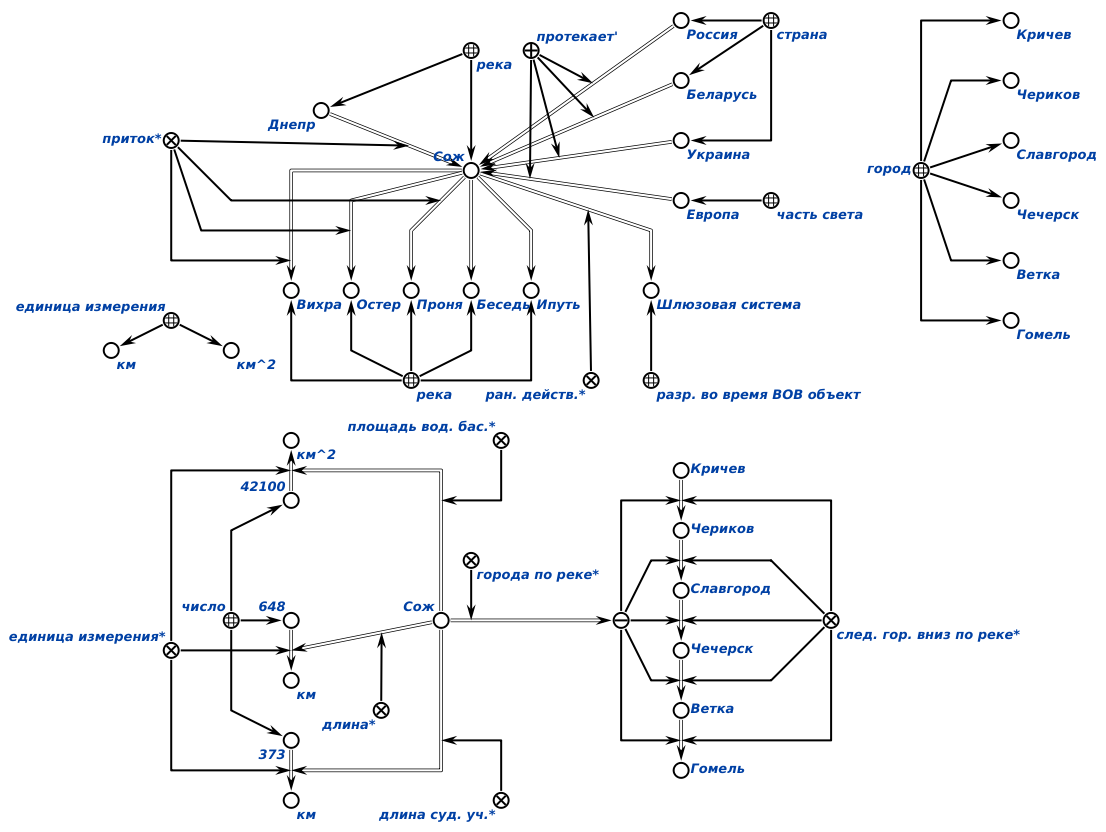
\includegraphics[scale=0.5]{images/work.png}
        }
    \scnaddlevel{-1}
    ~\\~\\~\\~\\
    \scnhaselement{Пример формализации на SCg №2}
    \scnaddlevel{1}
        \scntext{исходный текст}{ \(tg(3\alpha)=\frac{3tg\alpha-tg^{3}\alpha}{1-3tg^{2}\alpha}\) }
        \scnrelfrom{SCg}{
            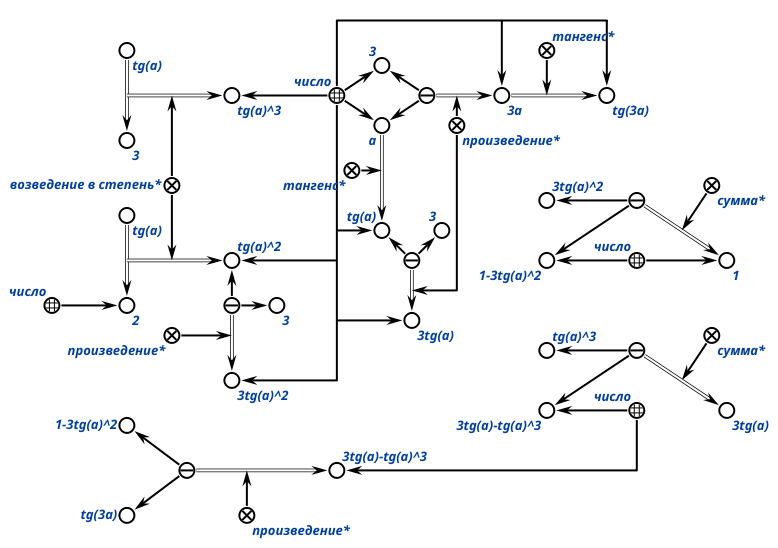
\includegraphics[scale=0.7]{images/work2.png}
        }
    \scnaddlevel{-1}
    \pagebreak
    \scnhaselement{Пример формализации на SCg №3}
    \scnaddlevel{1}
        \scntext{исходный текст}{ \(V = \frac{1}{3}{\pi}h(r^2_1+r_1r_2+r^2_2)\) }
        \scnrelfrom{SCg}{
            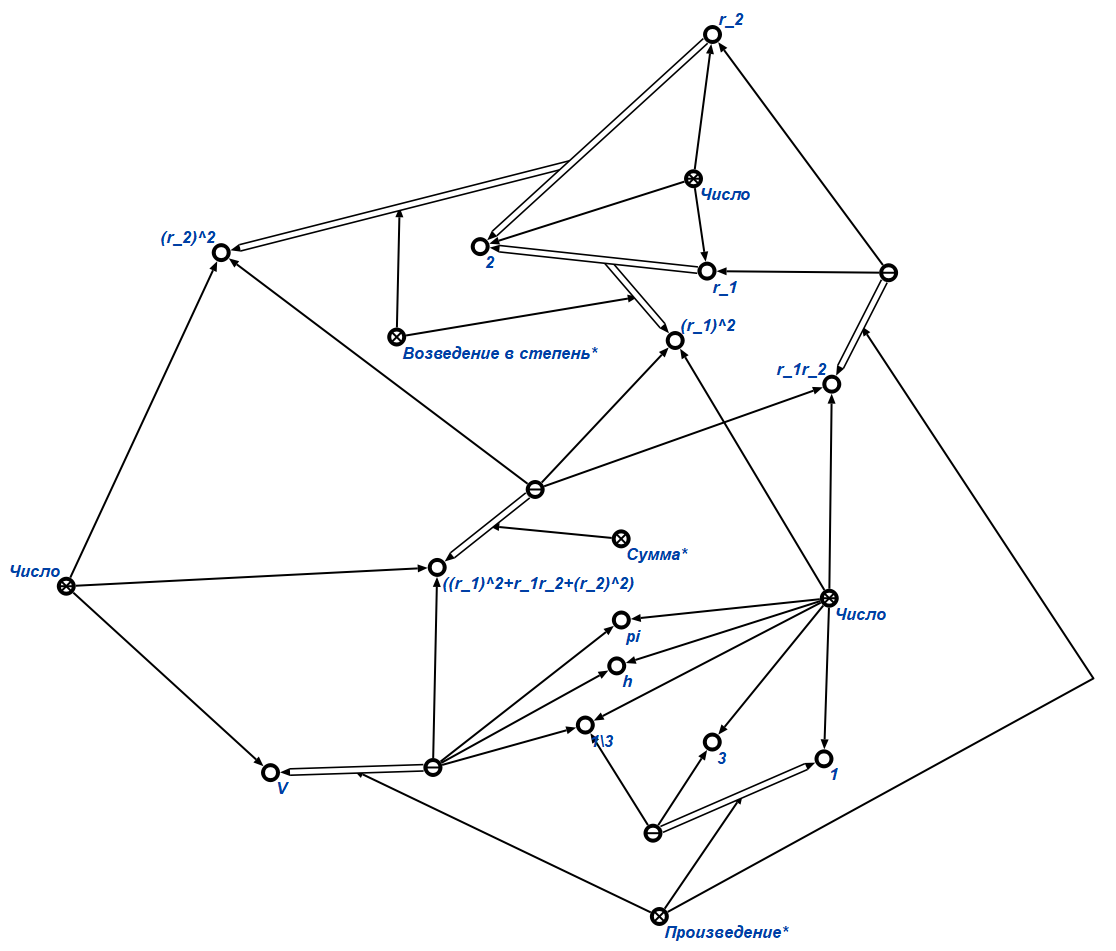
\includegraphics[scale=0.7]{images/ytsu.png}
        }
    \scnaddlevel{-1}
    \pagebreak
    \scnhaselement{Пример формализации на SCg №4}
    \scnaddlevel{1}
        \scntext{исходный текст}{Дан треугольник АВС. Периметр треугольника АВС равен 20 см. MN – средняя линия, параллельная стороне АС. MN лежит против угла B, градусная мера которого составляет половину градусной меры угла С. Медиана BK пересекает MN в точке О, АО = СО.}
        \scnrelfrom{SCg}{
            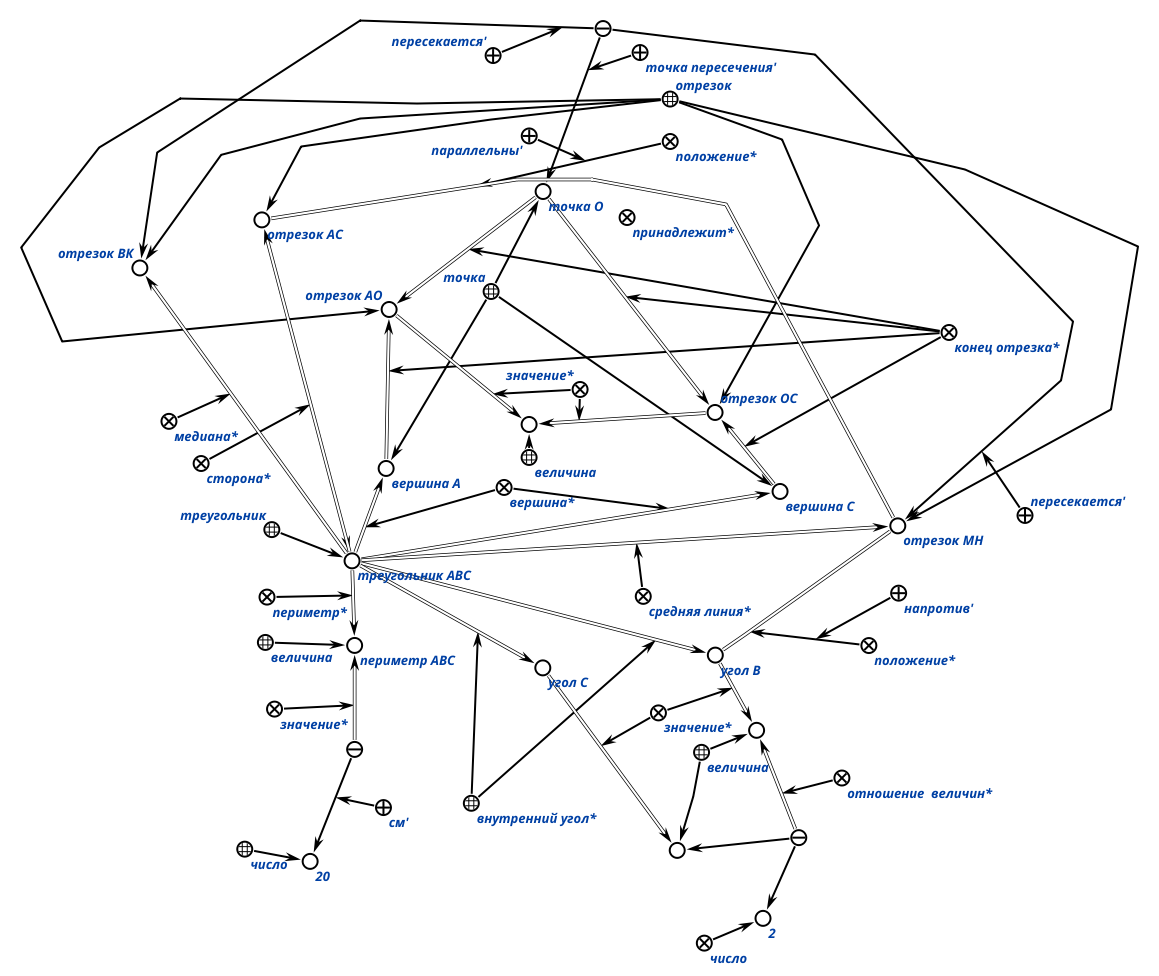
\includegraphics[scale=0.5]{images/sr.png}
        }
    \scnaddlevel{-1}
\end{SCn}

\newpage
\section*{Заключение}
\addcontentsline{toc}{section}{Заключение}

Построены формализованные фрагменты теории интеллектуальных систем и технологий, а именно: раздел о многократно используемых компонентах интеллектуальных систем, раздел о решателях задач -- с использованием языка внешнего представления баз знаний SCn (Semantic Code natural). Проведена работа по определению и пояснению сущностей, описанных в вышеприведенных разделах Стандарта OSTIS при помощи построения формальной семантической спецификации библиографических источников, а также внесены предложения в Стандарт примеров формализации на языке SCg (Semantic Code graphics).


% Если в тексте записки есть приложения, для добавления их в содержание, необходимо оставить слудеющую строку
% Если приложений нет - данную строку добавляем в комментарий
\addcontentsline{toc}{section}{Список использованных источников}

\nocite{*}
\bibliography{bibliography}


\end{document}
